%%%%%%%%%%%%%%%%%%%%%%%%%%%%%%%%%%%%%%%%%%%%%%%%%%%%%%%%%%%%%%%%%%%%%%%%%%%%%%%%
%characterization.tex: Chapter on ground characterization measurements:
%%%%%%%%%%%%%%%%%%%%%%%%%%%%%%%%%%%%%%%%%%%%%%%%%%%%%%%%%%%%%%%%%%%%%%%%%%%%%%%%
\chapter{Detector Characterization}
\label{sec:detector_characterization}
%%%%%%%%%%%%%%%%%%%%%%%%%%%%%%%%%%%%%%%%%%%%%%%%%%%%%%%%%%%%%%%%%%%%%%%%%%%%%%%%

%\textcolor{red}{If you are going to insist on referring to wafers by their names, you need to explain what the name means.}


%\textcolor{red}{You say in EACH of these cryostats the wafer was mounted and coupled to readout electronics as was done for flight. BUT. At McGill, it was only until the end of the copper pigtail that it was flight-like. So. That sentence isn't true. Unless you're being more general. It was connected to a strip that went to a squid that went to some cables (none of which were specific to ebex)... FIXED sentence.}

There were more than four dozen detector wafers fabricated and characterized for \ac{EBEX}. 
The wafer naming convention was \textit{frequency band - position in fabrication sequence}, e.g. 250-04 was the fourth 250~GHz wafer to be fabricated.
The characterization measurements were performed in testbeds designed to be as similar to the final flight configuration as possible. 
The three testbeds used were: 
a dedicated \ac{ETC}  at the University of Minnesota, %\ac{EBEX} test cryostat at the University of Minnesota, 
a test cryostat at McGill University, and the \ac{EBEX} cryostat itself, made dark. 
In the measurements reported here, the wafer was mounted and coupled to the readout electronics as was done for flight, Section~\ref{sec:ebex}. 
The wafers were cooled to 250-320~mK, where the exact temperature depended on the testbed. 
%highlight the difference between the light and dark configuration (and that you were attempting to minimize such that they were tested under conditions as similar to operation as possible.

As the fabrication procedure was modified to build detectors optimized for a space-like environment, we measured the detector parameters in the dark cryostats to provide feedback to fabrication. 
The detector parameter measurements also enabled us to estimate the sensitivity the detectors would be able to achieve. 

%%%%%%%%%%%%%%%%%%%%%%%%%%%%%%%%%%%%%%%%%%%%%%%%%%%%%%%%%%%%%%%%%%%%%%%%%%%%%%%%
% Parameter Measurements {{{
%%%%%%%%%%%%%%%%%%%%%%%%%%%%%%%%%%%%%%%%%%%%%%%%%%%%%%%%%%%%%%%%%%%%%%%%%%%%%%%%
\section{Detector Parameter Measurements}
\label{sec:parameter_measurements}
%%%%%%%%%%%%%%%%%%%%%%%%%%%%%%%%%%%%%%%%%%%%%%%%%%%%%%%%%%%%%%%%%%%%%%%%%%%%%%%%

The main detector parameters measured for each detector were normal resistance, critical temperature, and thermal conductance. 
For a subset of wafers, we also measured time constants, both electrothermal and optical. 
There was a dedicated cooldown in \ac{ETC} to measure the optical efficiency of some 150~GHz detectors. 

%%%%%%%%%%%%%%%%%%%%%%%%%%%%%%%%%%%%%%%%%%%%%%%%%%%%%%%%%%%%%%%%%%%%%%%%%%%%%%%%
\subsection{Normal Resistance}
\label{sec:normal_resistance}
%TOWARDS NORMAL RESISTANCES
%%%%%%%%%%%%%%%%%%%%%%%%%%%%%%%%%%%%%%%%%%%%%%%%%%%%%%%%%%%%%%%%%%%%%%%%%%%%%%%%

%\textcolor{red}{What exactly are you trying to say here? What is the point of this section? SEE BELOW.}

%\textcolor{red}{Are you going to include a zoom of one of the peaks. You would do this so you can show how (well) it fits to a Lorentzian and also to point out where you set the carrier frequency. do these plots already exist? hmmm. that must have been later in life when we saved the zooms of the fits? - REMADE}

%\textcolor{red}{You took this data, but you didn't write the code to make the plots. See: Kevin's thesis. So. Do you go back and remake the plots then??? Fuck. You're so far removed from this, you don't even remember how specifically you analyzed this data. YES, REMAKE.}

%\textcolor{red}{If you have time, it sure would be nice to go back and make those axes (the labels and the numbers) large enough to read. also, do in kHz. and use fewer words (more readable).}

%\textcolor{red}{You need a circuit diagram. BUT. Do you need to repeat the circuit diagram with a stray L and C?? No. I don't think so. People can add those two components in their heads??? INCLUDED IN INTRO SECTION. AND DECLINED TO INCLUDE THE ONE WITH LX AND CX.}


%Still want. But. Need to move on for now. COME BACK IF YOU HAVE TIME
%\textcolor{red}{I want you to mention how you determined the lower and upper bounds of the bias frequencies. And how you set the spacing. BUT. How did we do this??? I forget. Where is this information? SEE PAGE 9 (UPPER LEFT) OF DOBBS 2012 PAPER!}
%
%\textcolor{red}{Also, I want you to say (BUT IS THIS NECESSARY?), in practice, how did we match the frequencies measured with the frequencies \textit{expected}? The game. The measured frequency was generally XXX\% higher than the expected one calculated from the inductance measured at 4.2~K of $24~\mu H$ and the room temperature measured capacitances. At low frequencies, the measured frequency was close to expected. At the highest frequency, however, the measured frequency was nearly 90 kHz greater than expected. }
%
%\textcolor{red}{are you going to say which capacitors you used? specifically brands? values? are you going to talk about measuring the Ls? what about the setup designed just to do that?}
%
%\textcolor{red}{I want you to include: Typical stray capacitance was about XXX $pF$ and typical stray inductance was XXX $uH$. You'll also need to comment on the effect of having strays at this level, i.e. what does it do?? how much does it alter the voltage bias provided to the detector? cross-talk? }
%
%\textcolor{red}{Include: Stray impedance measured from an iv curve of a latched/superconducting bolometer.}
%
%\textcolor{red}{Fix reference to eqn:noisebudget}

%YOU DON'T REMEMBER THIS WELL ENOUGH TO TALK ABOUT IT
%AND SEARCHING EMAIL AND WEB AND READING THESES DIDN'T HELP ENOUGH
%We wanted to maximize the number of detectors per comb while minimizing harmful effects like cross-talk and whatever bad thing happens at low frequencies and whatever bad thing happens at high frequencies. 
%The lower end of the frequencies we could demodulate at was set by XXX and the higher end was set by XXX. 
%The inter-detector spacing was set by XXX. 
%We could wire up to 16 detectors per comb. 

In order to get the bolometer resonant frequencies and their normal resistances, we performed a network analysis on each comb with the bath held a couple hundred millikelvin above the critical temperatures.
The network analysis swept a voltage across the comb in frequency and measured the current response of the circuit, Figure~\ref{fig:network_analysis}. 
At each bolometer's LC resonant frequency, the multiplexed LCR circuit peaked in current. 

\begin{figure}[htbp]
\begin{center}
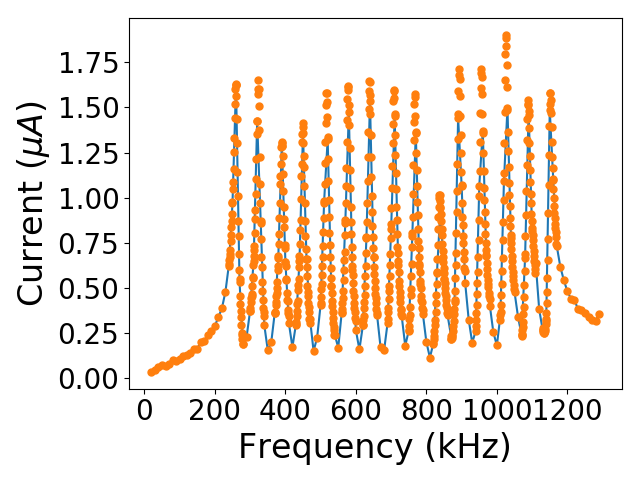
\includegraphics[width=0.6\columnwidth]{figures/SqCh3_netanal.png}
\caption{An 800~mK network analysis from wafer 150-17. The blue line has frequency steps of 10~kHz to roughly locate the peaks and the orange dots are finer scans with steps of 1~kHz to obtain the data to fit. 
\label{fig:network_analysis} }
\end{center}
\end{figure}

The impedance as a function of frequency, $\nu$, for each bolometer in series with its inductor, $L=24~\mu H$, and capacitor, $C_{i}$, was modeled as
\begin{equation}
Z_{LCR_{i}} \left(\nu\right) = \sqrt{ R_{i}^{2} + \left(2\pi \nu L - \frac{1}{2\pi \nu C_{i}}\right)^{2}}
\end{equation}
where $R_{i}$ was the $i^{th}$ bolometer's resistance.
There was also a stray inductance, $L_{x}$, and stray capacitance, $C_{x}$, in parallel with the detector comb. 
The network analysis current for each peak was thus
\begin{equation}
I = \frac{V_{bias}}{\lvert Z_{LCR_{i}} + j 2\pi \nu L_{x} + \frac{1}{j 2\pi \nu C_{x}}\rvert}
\end{equation}
Figure~\ref{fig:netanal_fit} shows a single peak and the fit to the model.
Note, the frequency at the maximum current and the optimal bias frequency are not necessarily aligned because we wanted to maximize the current through the bolometer rather than maximize the current through the entire circuit (which included the stray capacitance and inductance).

\begin{figure}[htbp]
\begin{center}
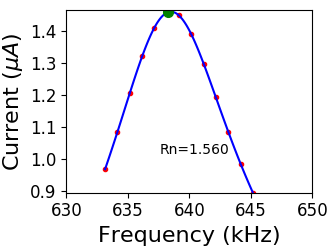
\includegraphics[width=0.3\columnwidth]{figures/netanal_etcsqb_SqCh3_10K_20110606_5to8.png}
\caption{The Lorentzian fit (blue line) to a network analysis peak (red dots). The fit provides the bolometer resonant frequency (green dot), the bolometer normal resistance, and the circuit's stray inductance and stray capacitance. 
\label{fig:netanal_fit} }
\end{center}
\end{figure}

Around 800~mK, when both the niobium leads on the wafer and the aluminum wirebonds between the wafer and the \ac{LC} board were superconducting, the fit provided the normal resistance of the \ac{TES}. 
%fitting the peak width provided the normal resistance of the \ac{TES}. 
Histograms summarizing the measured normal resistance values for the flight wafers, broken down by frequency band, are shown in Fig.~\ref{fig:rn_histograms}. 
%Section~\ref{sec:detector_optimization}. the optimization section doesn't actually provide the detail I want it to provide.
The median normal resistance, $R_{normal}$, for the 150, 250, and 410~GHz bands was 1.9, 1.5, and 1.0~$\Omega$ respectively. 
%\textcolor{red}{FROM THE PAPER.}
The 150 and 410~GHz bimodal distributions were due to detector parameters being closely grouped within a single fabrication run, but varying between fabrication runs. 
The measured value of $R_{n}$ for the 250~GHz band closely matched the design (see 
Table~\ref{tab:Design_Params}). 
For the other two frequency bands, one mode of the distribution closely matched while the other mode was higher (lower) than design for the 150 (410)~GHz band. 
The 150~GHz detectors with a measured $R_{n}$ of 1.9~$\Omega$, instead of the nominal 1.5~$\Omega$, were calculated to have increased electrical cross-talk from a value of 0.5\% to 0.9\% and decreased loopgain by 30\%. 
The 410~GHz detectors with a measured $R_{n}$ of 1~$\Omega$, two-thirds of the design value, were calculated to have increased Johnson noise by 20\% relative to the nominal expected value of 4.0 pA$/\sqrt{\mathrm{Hz}}$ (9.4~aW$/\sqrt{\mathrm{Hz}}$); see Equation~\ref{eq:johnson}.

\begin{figure}[ht!]
\centering
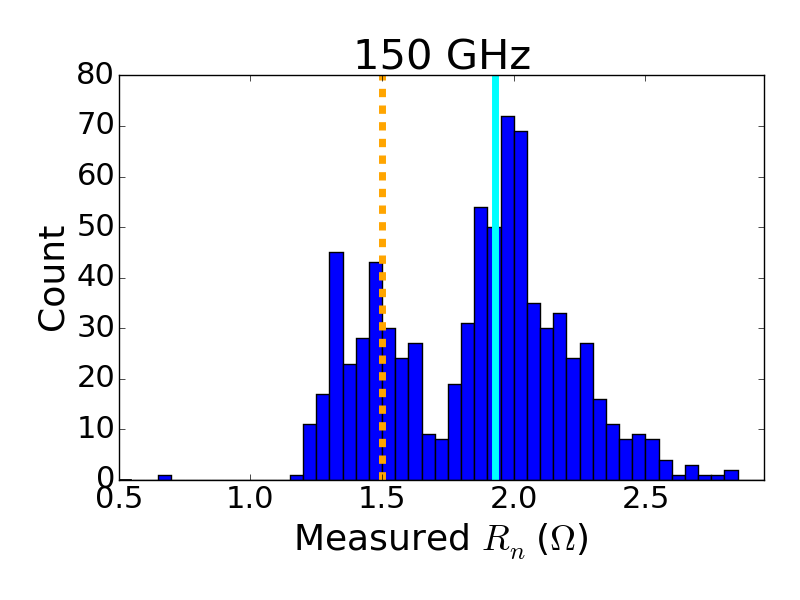
\includegraphics[width=0.32\textwidth]{figures/150_rn_hist.png}
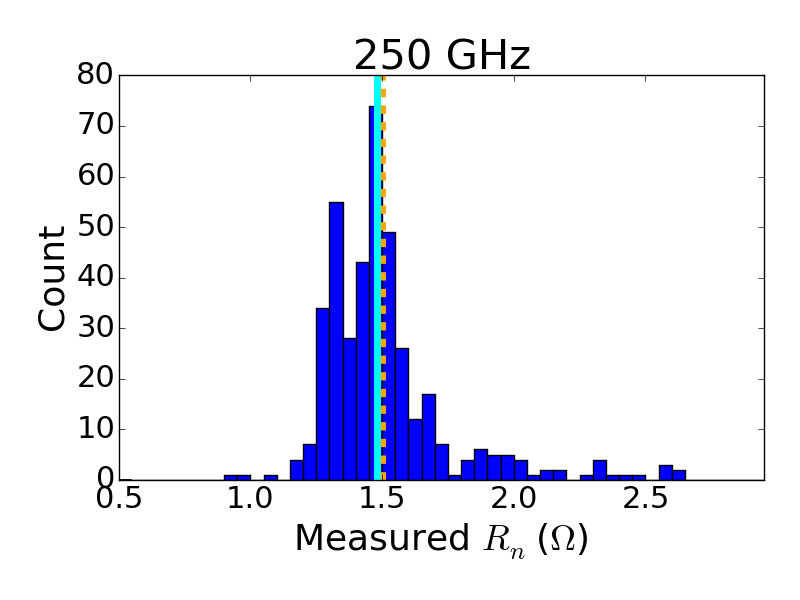
\includegraphics[width=0.32\textwidth]{figures/250_rn_hist.png}
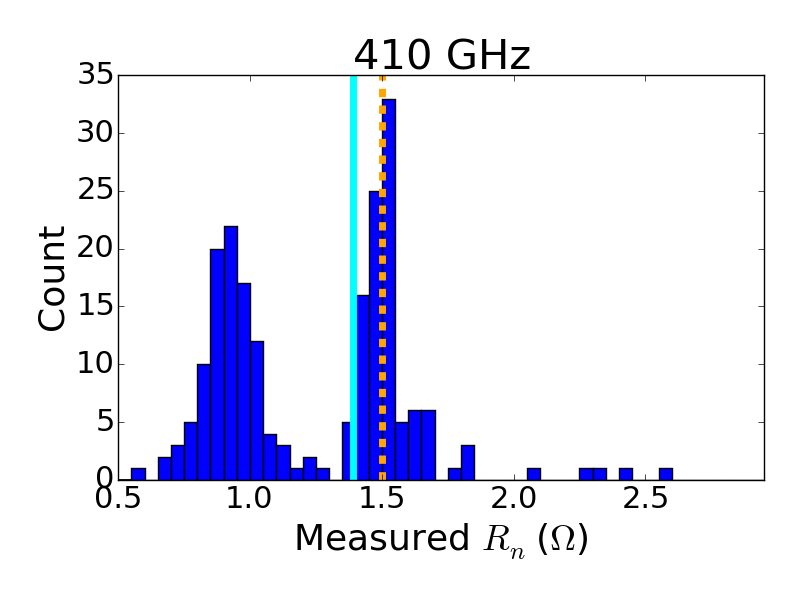
\includegraphics[width=0.32\textwidth]{figures/410_rn_hist.png}
\caption{Histogram of measured normal resistances $R_{n}$ for each of the frequency bands, including the median (vertical cyan)  
and design (vertical gold dashed) values.
\label{fig:rn_histograms} }
\end{figure}





%\textcolor{red}{again, I'd like you to remake this figure so the units and axes across figures are consistent ... this one says "f (kHz)", the other says "Carrier Frequency (Hz)"}

%YOU DON'T GET TO INCLUDE THIS??? 
%YOU DIDN'T WRITE THE FITTING OR PLOTTING CODE
%\begin{figure}[htbp]
%\begin{center}
%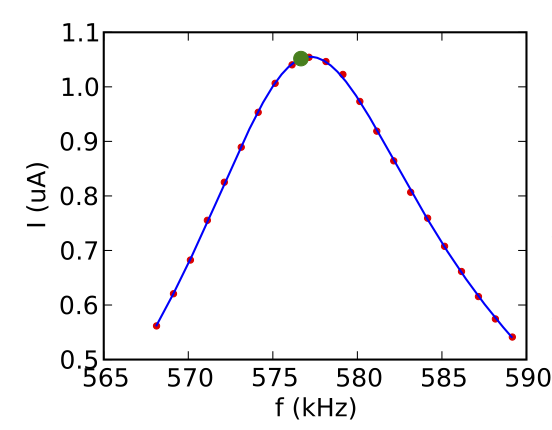
\includegraphics[height=2in]{figures/netanal_zoom.png}
%\caption{The fit of a network analysis peak (blue solid) to a Lorentzian and the optimal bias frequency determined (green dot).
%\label{fig:network_analysis_zoom} }
%\end{center}
%\end{figure}


%The consequences of overshooting this value, as is the case for many of the 150~GHz detectors, are an increase in the detector voltage bias leakage, which is proportional to $R^2$ \cite{dobbs_revSciInst_2012}, and a decrease in the loopgain, which is inversely proportional to R. 
%% if R is higher, then johnson current noise is decreased since it goes like 1/sqrt(R)
%% if R is higher, then stability requirement has R/(2*pi*L) > 5.8/tau_tes is more satisfied
%For a detector dropped to 85\% in the transition, having a normal resistance of 1.9~$\Omega$ instead of 1.5~$\Omega$ results in a bias leakage increase of 60\%, increasing the cross-talk from 0.5\% to 0.8\%, and a loopgain decrease of 30\%. 
%The consequence of undershooting the normal resistance, as is the case for many of the detectors on wafer 410-28, is an increase in the Johnson current noise. The Johnson noise is proportional to $1/\sqrt{R}$, so that noise term increases by 20\% given a value of 1.0~$\Omega$ instead of 1.5~$\Omega$.



%\comred{Assume detector optimization explains what about the electronics set our target to be 1.5~$\Omega$? Ben says "The requirement is really ~1.25 because what actually matters is Rtes in transition for the L/R requirement.  So depending on how deep we get in to the transition we could start anywhere just above 1.2 Ohms to operate at 0.88 to 1.0 Ohms." BUT. When determining which Rfrac to tune to, we didn't do this calculation. Rather, we noted, in general, below 80\% $R_{start}$, we had (not well understood) excess noise and so opted to go to 85\%. What I'm trying to say is, in practice, the operating fracRn value was not chosen carefully on a bolo by bolo basis or even a wafer by wafer basis to achieve a specific L/R. Explain the consequence of having a higher or lower normal resistance, e.g. 150s and one of the 410s (was it the 410 that operated or the 410 that was saturated?)? Ben says "Increased johnson noise and possibly bolo stability.  However, I'm not sure if either of these effects were detected in the wafers in test cryostats, Palestine, or flight."}



%%%%%%%%%%%%%%%%%%%%%%%%%%%%%%%%%%%%%%%%%%%%%%%%%%%%%%%%%%%%%%%%%%%%%%%%%%%%%%%%
\subsection{Critical Temperature}
\label{sec:critical_temp}
%TOWARDS CRITICAL TEMPERATURES
%%%%%%%%%%%%%%%%%%%%%%%%%%%%%%%%%%%%%%%%%%%%%%%%%%%%%%%%%%%%%%%%%%%%%%%%%%%%%%%%

%\textcolor{red}{HAVE WE MOTIVATED ELSEWHERE WHY WE CARE ABOUT VALUE OF $T_{C}$? Yes.}

%
%WOULD LIKE TO ADDRESS THESE! COME BACK IF YOU HAVE TIME. 
%\textcolor{red}{WANT WARMING AND COOLING IN ETC. BE CLEAR ABOUT HYSTERESIS FROM WARMING AND COOLING. I'd like for you to note we need to perform this slowly because there is an inherent hysteresis, LAG DUE TO TEMPERATURE SENSOR BEING MOUNTED TO INVAR INSTEAD OF TES.}
%
%\textcolor{red}{Note, this resistance does not agree with the resistance measured via the network analyses or via the IV curves. Any ideas why? Maybe bring this up in loopgain section???}
%
%\textcolor{red}{Is it worth nothing there is a resistance offset of $\sim 0.1 \Omega$? And this tells us something about our stray impedance?}
%
%\textcolor{red}{Can you explain exactly how $T_{c}$ was extracted from the data, i.e. what temperature did you call Tc? Also, what defined/determined the transition width?}

For the measurement of the critical temperature in \ac{ETC}, we placed a voltage bias of 5~$nV_{rms}$ across the detector such that the Joule heating of $\frac{V^2}{R} = 1.5~fW$ was negligible but there was still a measurable current signal. 
The temperature was slowly, less than 3~mK/min, dialed up and down to move the bolometers through their superconducting transitions. 
Changing the temperature slowly was important because the temperature was read out from a sensor attached to the underside of the invar plate onto which the wafer was mounted 
%2. the wafer heater was mounted to the underside of the invar. 
and the bolometers were only weakly coupled to the bath via their spiderweb legs. 
We used the bath temperature as a proxy for the bolometer temperature. 
%I WANT YOU TO SAY WHY IT WAS IMPORTANT TO DO THIS MEASUREMENT DARK (COME BACK IF YOU HAVE TIME)
Without time to thermalize, there would have been significant hysteresis. 
This measurement also relied on the cryostat being dark because radiative power would have increased the temperature of the detector but not the bath where the temperature sensor was mounted. 
%So the wafer temperature sensor would not have been a good proxy for the bolometer temperature. 
Fig.~\ref{fig:tc_measurement} is an example of a critical temperature measurement for a bolometer on wafer~150-02. 
We measured demodulated \ac{ADC} counts with the \ac{DfMUX} boards and converted to resistance using the measured current and voltage transfer functions and Ohm's law, $R=V_{bias}/I_{measured}$.
When the \ac{TES} was superconducting, there was an offset in the resistance measured because there was still current due to the non-zero stray impedance. 
%When the \ac{TES} is normal, there is more noise because .... why would the current be noisier when the \ac{tES} was normal ??? current was smaller. so we saw digitization noise?


%The bottom two panels show the bolometer resistance as a function of time and temperature. 
%The hysteresis between the critical temperature measured cooling and warming is generally less than 5~mK, sufficiently accurate for characterization.

\begin{figure}[htbp]
\begin{center}
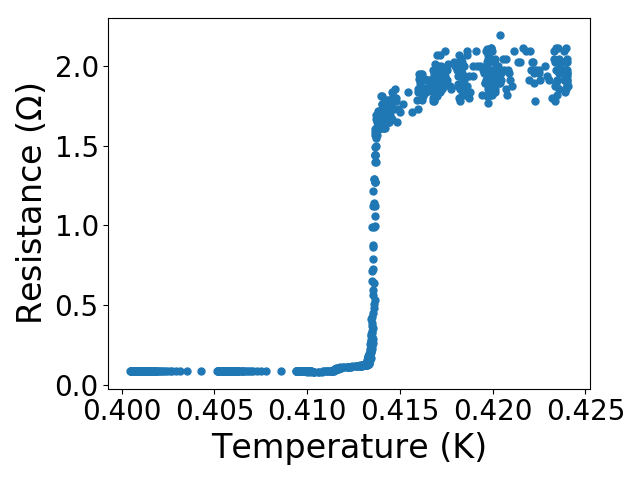
\includegraphics[height=2.5in]{figures/b53w0c0_rvst.png}
\caption{Resistance as a function of bolometer temperature for a detector from wafer 150-02. The resistance was the ratio of the voltage bias across the bolometer to the current measured through the \ac{SQUID}. This bolometer had a $T_{c}$ of $\sim$414~mK. 
\label{fig:tc_measurement} }
\end{center}
\end{figure} 

Histograms summarizing the measured critical temperatures for the three \ac{EBEX} frequency bands are shown in Fig.~\ref{fig:tc_histograms}. 
%The target critical temperature for each band was 0.44~K, a value which optimizes the phonon noise term given the \ac{EBEX} bath temperature. %or refer to Section~\ref{sec:detector_optimization} for the motivation ??
The median critical temperatures, 0.45, 0.49, and 0.51~K for the 150, 250, and 410 GHz bands, respectively, were within 16\% of the target value of 0.44~K. 
%There was a $\sim$20\% wafer-to-wafer spread
The greatest spread in measured values of $T_{c}$ was in the 150~GHz band. 
The effect of this spread is to increase Johnson (phonon) 
noise when $T_{c}$ is above (below) the design value. 
At the high (low) edge of the distribution with $T_{c}$~=~0.54~K (0.36~K), there was an 11\% (5\%) increase in the calculated Johnson (phonon) noise 
relative to the nominal expected value of 4.0~pA/$\sqrt{\mathrm{Hz}}$ (20~aW/$\sqrt{\mathrm{Hz}}$). 


%IN THE PAPER, THEY GO ON TO TALK ABOUT THE EFFECT OF THE MEASURED TCS ON PSAT AND RESPONSIVITY, BUT IT'S NOT MAKING SENSE TO ME AND I DIDN'T DO THE CALCULATION. COME BACK TO THIS IF YOU HAVE TIME.

%The consequence of overshooting the critical temperature, as for some of the detectors in each of the frequency bands, is an increase in the Johnson noise, proportional to $\sqrt{T}$, and an increase in the phonon noise, proportional to $T$. 
%The consequence of undershooting the critical temperature, as for roughly half of the 150~GHz detectors, is potentially not being able to drop the detector into the transition because the critical temperature is too close to the bath temperature. % is this actually why we didn't want to go too low?
%\comred{what's the consequence of the wide spread in Tc for the 150s? how concerned are we about the level of spread we fabricated?}

%FROM THE PAPER.
%There was a $\sim$20\% wafer-to-wafer spread in the measured $T_{c}$ with the medians for the three bands within 
%16\% of the target value of 0.44~K. 
%The 150~GHz detectors have the widest spread of measured $T_{c}$. The effect of this spread is to increase Johnson (phonon) 
%noise when $T_{c}$ is above (below) the design value. 
%At the high (low) edge of the distribution with $T_{c}$~=~0.54~K (0.36~K), there was an 11\% (5\%) increase in the calculated Johnson (phonon) noise 
%relative to the nominal expected value of 4.0~pA/$\sqrt{\mathrm{Hz}}$ (20~aW/$\sqrt{\mathrm{Hz}}$). 



\begin{figure}[ht!]
\centering
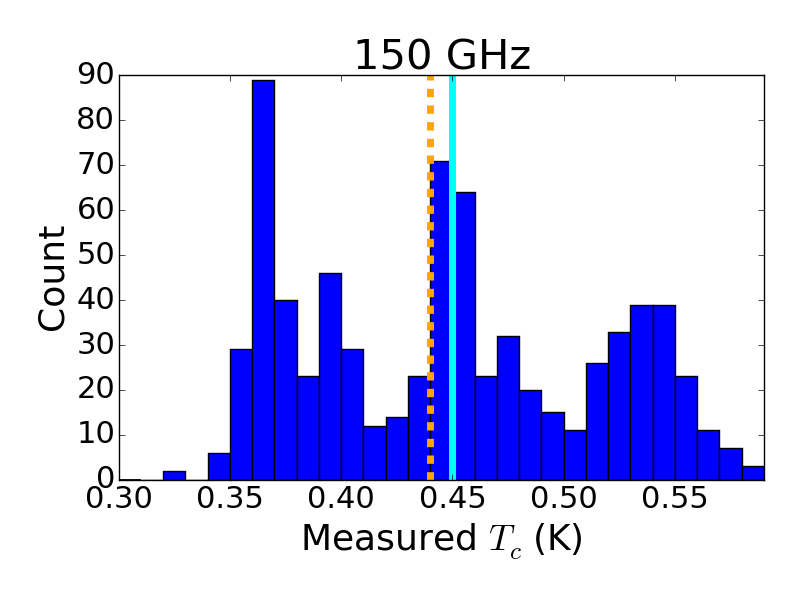
\includegraphics[width=0.31\textwidth]{figures/150_tc_hist.png}
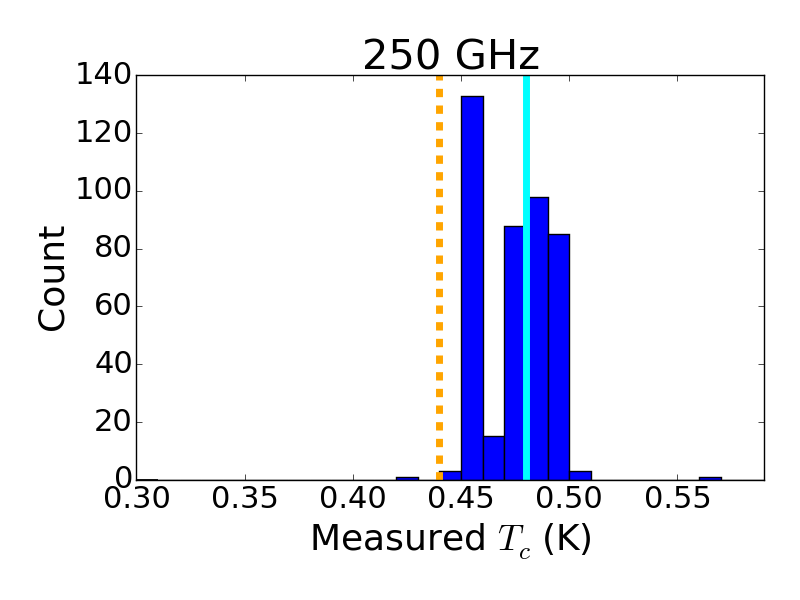
\includegraphics[width=0.31\textwidth]{figures/250_tc_hist.png}
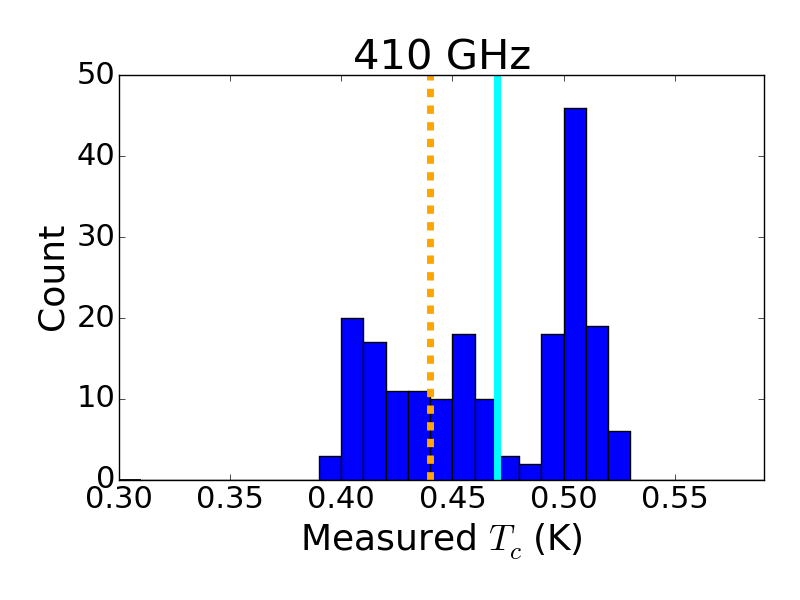
\includegraphics[width=0.31\textwidth]{figures/410_tc_hist.png}
\caption{Histogram of measured critical temperature values for the detectors in each frequency band including the median (vertical cyan) and design (vertical gold dashed) values. 
\label{fig:tc_histograms} }
\end{figure}


%%%%%%%%%%%%%%%%%%%%%%%%%%%%%%%%%%%%%%%%%%%%%%%%%%%%%%%%%%%%%%%%%%%%%%%%%%%%%%%%
%\subsection{Red Text}
%%%%%%%%%%%%%%%%%%%%%%%%%%%%%%%%%%%%%%%%%%%%%%%%%%%%%%%%%%%%%%%%%%%%%%%%%%%%%%%%


%\textcolor{red}{will you have already discussed \ac{NEP}? Yes. In 2.1. Bolometer Theory. in particular, phonon noise. for now point to eqtn in measured noise section.}

%\textcolor{red}{you need to be clear that you are using noise and \ac{NEP} interchangeably. NO. They are not interchangeable. Stop using them as if they were.}

%\textcolor{red}{Address: Why do we need to know the thermal conductance? i.e. Why do we care? When we talked about targets, we already should have talked about including a safety factor? And what set that target? maybe all of these words need to be moved to the bolometer theory section?}
% too vague. The thermal conductance of the thermal link from the TES to the bath governs the bolometer sensitivity. 

%\textcolor{red}{In bolometer theory, you need to have already explained electrothermal feedback.}

%COME BACK TO ALL OF THESE IF YOU HAVE TIME!

\textcolor{red}{How do we measure the thermal conductance? (Be sure you explain how we get from IV to PV and how we extract $P_{electrical}$ and how wrong we might be about this number.)}

\textcolor{red}{You need to say what bath temperature these average thermal conductances are quoted at and how you got them.}
\textcolor{red}{Are you going to include the Psat versus Tbath curves, for e.g. 150-02? They fit poorly to  $P = (a/l*kappa_{o})/(n+1)*[T_{c}^{n+1} - T_{o}^{n+1}]$. The fits don't look good on the plots and the uncertainty (presumably a standard deviation) on the fit is larger than the values.}

\textcolor{red}{Discuss results. What are the major uncertainties in this measurement? Talk about how deep you drop and how you define depth in transition. (will address noise as function of depth in transition in dark noise section).}
\textcolor{red}{Use this R vs V curve to help explain how deep in the transition the detectors are dropped. point out why it isn't the greatest way. Also, point out that R at high values of $V_{bias}$ still has some slope (how much slope?), so it's not obvious where to define $R_{normal}$. }
\textcolor{red}{Mention voltage bias is kind of a proxy for temperature? i.e. R vs V is effectively an R vs T curve where we don't have a calibration for the x-axis?}
\textcolor{red}{are you going to comment on how the resistance measured for this bolo (2.9 $\Omega$) compares to the resistance measured via the network analysis? put that information in a loopgain section instead?.}
\textcolor{red}{Talk about why it's not correct to do the ratio of vbias/imeasured and call that R? what uncertainty does this introduce?}

\textcolor{red}{You need to talk about going from average thermal conductance to dynamic thermal conductance ... does that belong here? no, I think it'd be better in bolometer theory or in the measured noise section. and it'll be fine if you also move the top paragraph out.} 
%Step one: introduce each one (in bolometer theory)
%step two: provide equation relating the two. 

\textcolor{red}{You need to comment on the $\overline{G}$ distribution shapes and consequences of overshooting, e.g. for 410~GHz.}
\textcolor{red}{What have we learned from the thermal conductance measurements? How did we (attempt to) modify detector fabrication given our measurements?}


%WOULD BE NICE TO HAVES
\textcolor{red}{Talk about the stray impedance effect you modeled. also, trevor lanting talked about this? in the case of a well-behaved bolometer with small stray impedance, \cite{Lanting2006}  }\textcolor{red}{I wish you could find or rewrite the code to make the bolo.iv.curve figures - the pW are in square brackets and all the others in parenthesis. and the axis labels are smaller than I want them to be.}
\textcolor{red}{are you going to comment on WHY the fit gives a non-zero current offset?}
\textcolor{red}{Do you want to include double transition iv curve? e.g. /data/ebex3/systems/nigel/data/2010/nigel.backup.data/07/30/boloIV.340mK/plots/250-01-02.IV.201007301208.png}
\textcolor{red}{Talk about dropping one bolometer at a time versus dropping the entire comb? i.e. talk about cross-talk? and how it's more dramatic when overbiased because the signal you're supplying is stronger?}
\textcolor{red}{ What happened when we measured $P_{elec}$ in ebex vs etc vs mcgill? How do we deal with different bath temperatures?}
\textcolor{red}{Doesn't it make sense to expand on the sources of radiative load? and instead of saying expected load, say exactly what the expected load was?}

%%%%%%%%%%%%%%%%%%%%%%%%%%%%%%%%%%%%%%%%%%%%%%%%%%%%%%%%%%%%%%%%%%%%%%%%%%%%%%%%
\subsection{Thermal Conductance}
\label{sec:thermal_conductance}
%TOWARDS THERMAL CONDUCTANCES 
%%%%%%%%%%%%%%%%%%%%%%%%%%%%%%%%%%%%%%%%%%%%%%%%%%%%%%%%%%%%%%%%%%%%%%%%%%%%%%%%

%The detector sensitivity is a function of the thermal conductance, $G$, of the link from the TES to the bath. %, Figure~\ref{fig:bolometer_cartoon}.
%In particular, the phonon \ac{NEP} is proportional to $G$, Equation~\ref{eq:phonon_nep}. 
%as well as any fluctuations in load %fluctuations are a problem for ground-based expt's, not us
The dark test cryostat measurements of the thermal conductance of the link from the \ac{TES} to the bath allowed us to predict the phonon \ac{NEP} for each detector and also determine if there would be sufficient dynamic range to operate the detectors under the expected loading conditions. 
We wanted to minimize $G$ so that we minimized the detector \ac{NEP} and thus maximized the detector sensitivity. 
The value of $G$, however, needed to be sufficiently high to allow for the detectors to operate in the presence of the radiative load at float, Section~\ref{sec:detector_design}. 

In order to measure the thermal conductance of the link, 
%we performed an IV curve for each bolometer.
%That is, 
we stepped down the voltage bias, typically in steps of 0.05~$\mu V$, and measured the current through the \ac{TES}. 
At each step, the instantaneous resistance, the ratio of the voltage bias to the current measured, was calculated, Figure~\ref{fig:bolo_rv_curve}. 
The bias voltage of each bolometer was dropped until the ratio of the voltage bias to the current measured reached a fixed fraction of its original value.
In the test cryostats, the fraction was typically 0.7. 
For \ac{EBEX2013}, the fraction was 0.85 for the majority of flight.
The value used in flight was higher than the nominal lab value because in the test cryostats the bolometer noise performance deeper in the transition diverged from the predictions, Section~\ref{sec:dark_noise}. 
%Note, in Figure~\ref{fig:bolo_rv_curve}, in the over-biased, normal region, the resistance of the bolometer has a non-zero slope. 

\begin{figure}[htbp]
\begin{center}
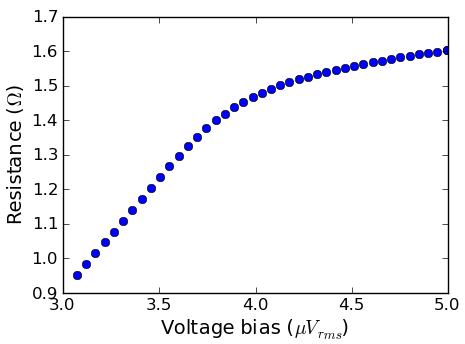
\includegraphics[height=2in]{figures/b53w0c0_RV.png} 
\caption{The instantaneous resistance ($I \over V$) of a 150-01 bolometer as a function of the voltage bias across the bolometer. This bolometer was dropped to 0.6 of the starting value. 
\label{fig:bolo_rv_curve} }
\end{center}
\end{figure}


The left panel of Figure~\ref{fig:bolo_iv_curve} is an IV curve, the current measured as a function of the voltage bias across the \ac{TES}, for one detector on wafer~150-01.
Above the superconducting transition, at higher voltage biases, the AlTi bilayer of the \ac{TES} was normal and so the current was proportional to $1/R$. 
Fitting the linear, normal region for this particular detector gave a resistance of 2.2~$\Omega$.
%I=0.45V+0.85 this one had a big offset! 
%RETURN HERE IF TIME
%Note this resistance value was XXX higher than the value found from the network analysis. 
As the bilayer began to superconduct, the resistance dropped and the current measured turned around. % with a characteristic smooth checkmark shape. NOT THIS PLOT!
Once the bolometer was sufficiently far into the superconducting transition, negative electro-thermal feedback kept the power dissipated in the bolometer at a fixed level, Section~\ref{sec:tes_bolometer}.
The right panel of Figure~\ref{fig:bolo_iv_curve} is a PV curve, the power dissipated in the bolometer ($I \times V$) as a function of the voltage bias. 
The electrical power required to hold the detector in the transition is the horizontal section of the PV curve, $\sim$10~pW for this detector.

\begin{figure}[htbp]
\begin{center}
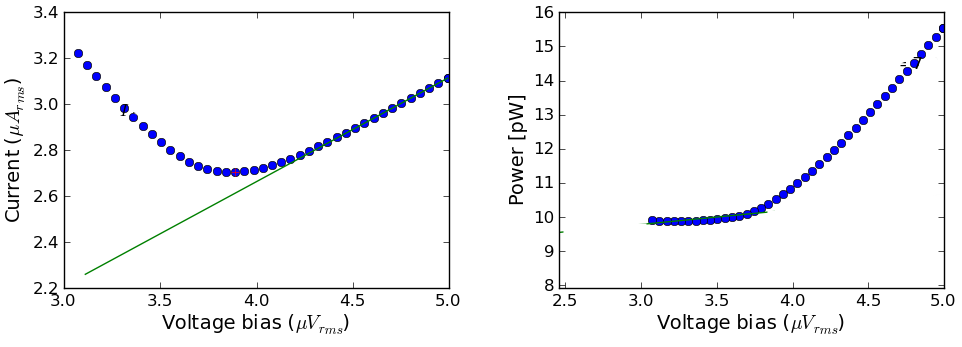
\includegraphics[width=0.99\columnwidth]{figures/b53w0c0_IV.png} 
\caption{Left: The current through the \ac{SQUID} as function of the voltage bias across the bolometer. Right: The electrical power dissipated in the bolometer ($I \times V$) as a function of the voltage bias across the bolometer.
\label{fig:bolo_iv_curve} }
\end{center}
\end{figure}

% RETURN TO THIS IF YOU HAVE TIME. 
%\begin{figure}[htbp]
%\begin{center}
%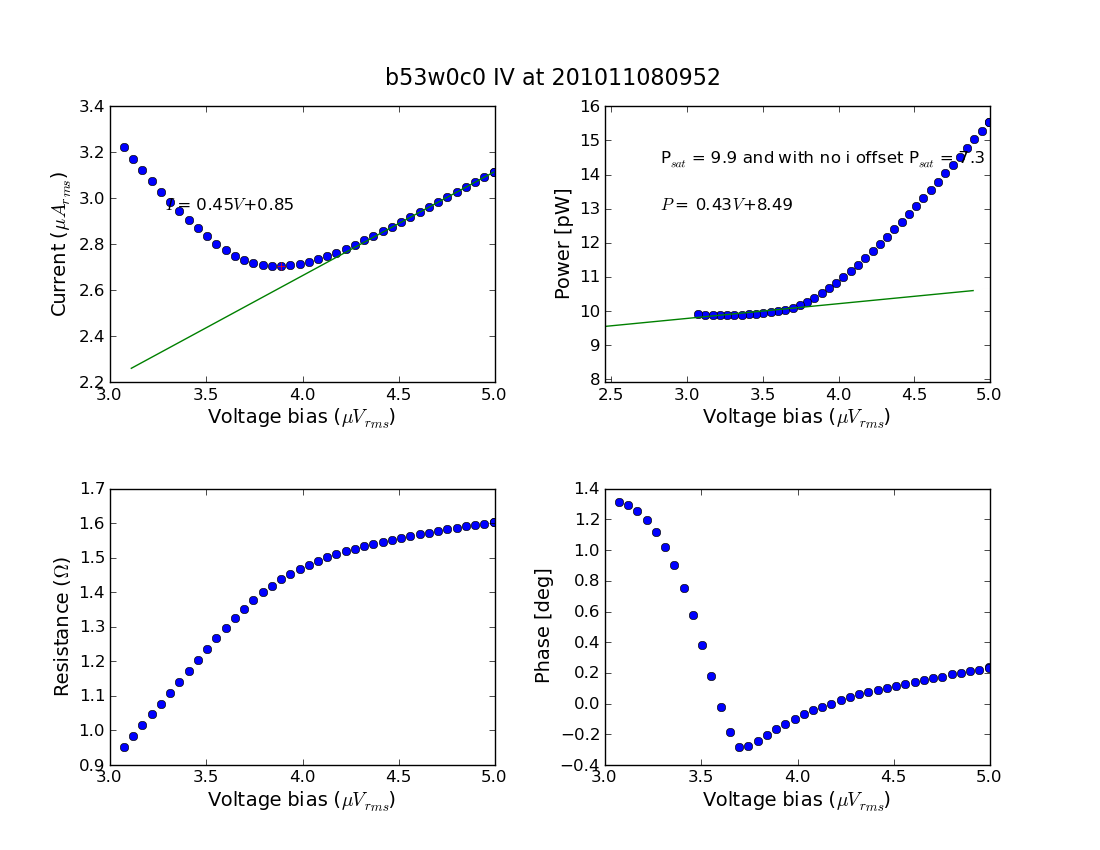
\includegraphics[width=0.99\columnwidth]{figures/b53w0c0_IV_201011080952.png} 
%\caption{Consider using this bolo's iv curve instead because it was dropped deeper in the transition.
%\label{fig:other_bolo_iv_curve} }
%\end{center}
%\end{figure}




%%%%%%%%%%%%%%%%%%%%%%%%%%%%%%%%%%%%%%%%%%%%
%RETURN TO THIS SECTION ON STRAY IMPEDANCE IF YOU HAVE TIME
%This is 150-02 b53w0c0 dropped to 60\% $R_{initial}$ using the IV algorithm which nulled at each voltage step and measured the current required to null the detector timestream.
%The green line is the naive calculation of power: P = I*V.
%The other lines include a stray imaginary impedance: $P = I^2*R, R = sqrt[(V/I)^2 - Rx^2]$
%teal has Rx = 0.2
%pink has Rx = 0.3
%blue has Rx = 0.33
%red has Rx = 0.4
%From this data, because we know the power dissipated in the bolometer deep in the transition is constant, we would conclude Rx ~ 0.3j ohms.
%This corresponds to a stray inductance of Lx ~ 110 nH. (used ZL = i*omega*L, and $\nu_{res} \approx 430~kHz$)
%For b53w0c0 at 60\% in the transition, Rbolo ~ 1.0 ohms. (calculated letting Rx = 0.3)
%The responsivity factor $sqrt[(1+eta^2)]/(1-eta^2) ~ 1.15$.
%A 15\% increase in the responsivity is not enough to explain the factor of 2.5 between the measured and predicted noise for b53w0c0 at 60\% in the transition.
%
%\begin{figure}[htbp]
%\begin{center}
%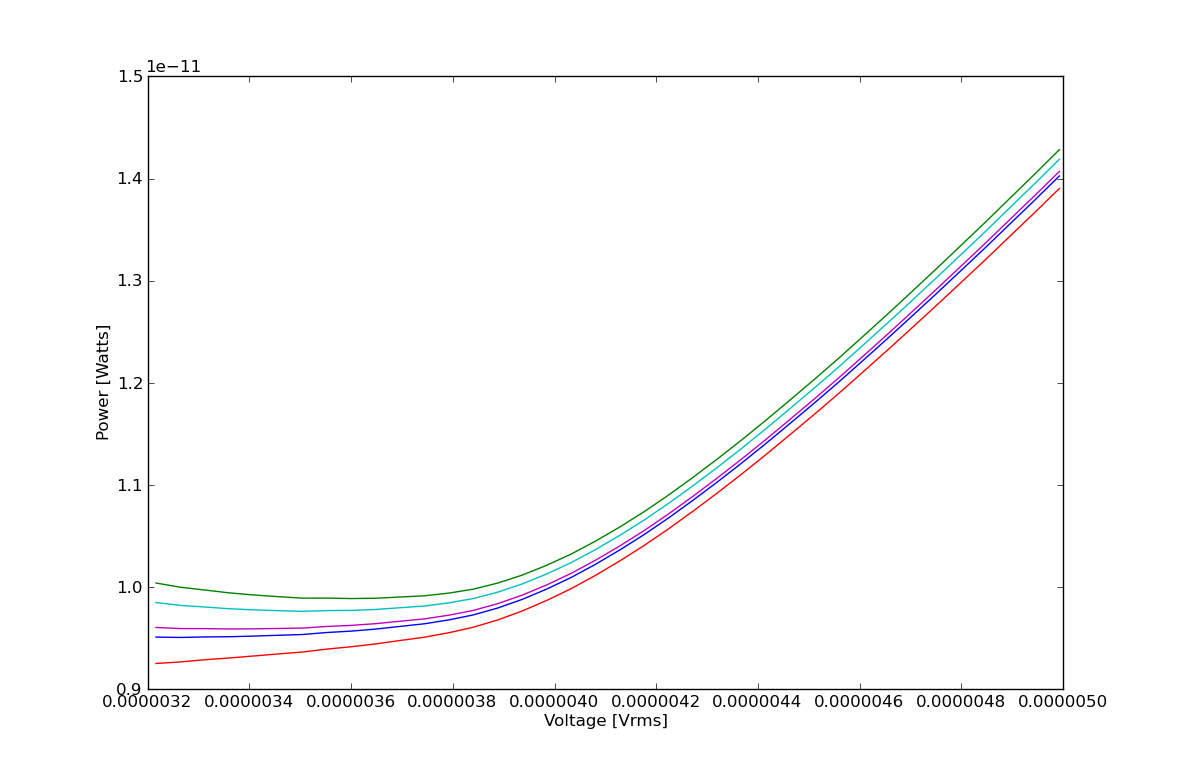
\includegraphics[height=2.5in]{figures/150-02_b53w0c0_messingwithX.png} 
%\caption{Simulating stray impedance.
%\label{fig:stray_impedance_curve} }
%\end{center}
%\end{figure}
%
%\begin{figure}[htbp]
%\begin{center}
%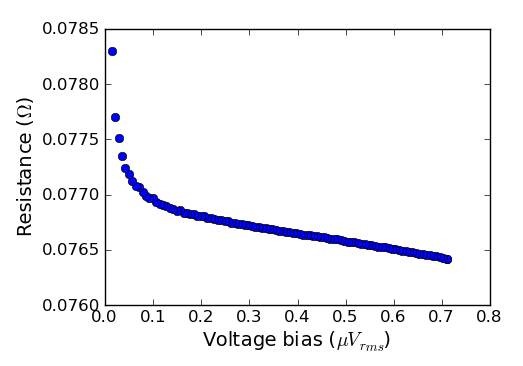
\includegraphics[height=2.5in]{figures/b53w0c0_IV_latched.png} 
%\caption{Measure of resistance while bolometer is superconducting. This channel has $R_{x} = 0.08 \Omega$ and we typically find $R_{x} \sim 0.1 \Omega$. Is this even a legitimate method to get stray impedance??? Are you measuring $R_{x}$? $Z_{x}$? Nothing of the sort?
%\label{fig:latched_iv_curve} }
%\end{center}
%\end{figure}
%%%%%%%%%%%%%%%%%%%%%%%%%%%%%%%%%%%%%%%%%%%%


%As the Joule Power decreases, the detector temperature decreases towards its transition temperature and the . 

For the dark characterization tests, because each bolometer wafer was enclosed in a light-tight box which was heat sunk to the bath, the radiative power on the bolometer should have been negligible. 
In the case of a negligible radiative load, the total electrical power measured from the PV curve was the total power dissipated in the detector. 
This power was often referred to as the saturation power, $P_{sat}$. 
%The detector in Figure~\ref{fig:bolo_iv_curve} has $P_{sat} = 1.9~pW$.
The saturation power was a useful parameter to think in terms of because the bolometer lost nearly all sensitivity if it saturated, i.e. if $P_{sat}$ was less than or near to the radiative load during observations. 

The average thermal conductance of the weak link for each detector was calculated from $P_{sat}$, measured from the PV curve, and its measured critical temperature, Section~\ref{sec:critical_temp}, 
\begin{equation}
\overline{G}(T_{bath}) = \frac{P_{sat}(T_{bath})}{T_{c} - T_{bath}}
\end{equation}
$\overline{G}$ is a function of the bath temperature. 
The test cryostats operated at different bath temperatures than \ac{EBEX}, so the measured $\overline{G}$s needed to be adjusted to the \ac{EBEX} bath temperature. 
%In order to calculate $\overline{G}$ for \ac{EBEX}, we assume XXX. 
If the phonon transport along the weak link was diffusive, as opposed to ballistic (where the mean free path of the phonon was much longer than the length of the material in the direction of travel), then the thermal conductivity followed a power law, 
\begin{equation}
\kappa \left( T \right) = \kappa_0 T^n
\end{equation}
where n was the power of the thermal conductivity. 
Normal metals have $n=1$ while crystalline dielectrics or superconductors have $n=3$ \cite{Mather1982}. 
The 2009 \ac{EBEX} test flight wafers were measured to have n values of 2.2 $\pm$ 0.3, 1.9 $\pm$ 0.2, and 2.1 $\pm$ 0.2 for the 150, 250, and 410~GHz bands respectively \cite{Hubmayr2009}.
If the weak link had a uniform cross section of area $A$ and length $l$, then the thermal conductance was 
\begin{equation}
G = \frac{A}{l} \kappa_0 T^n
\end{equation}
and the power flow was described by
\begin{equation}
P = \int \frac{dP}{dT} dT = \int_{T_{bath}}^{T_c} \frac{A}{l} \kappa_0 T^n dT = \frac{A\kappa_0}{l(n+1)} \left( T_c^{n+1} - T_{bath}^{n+1} \right)
\label{eq:power_int}
\end{equation}
Letting this equal equation~\ref{eq:gbar} and then taking the ratio of the power in \ac{EBEX} to the test cryostat, we found the corrected thermal conductance at the \ac{EBEX} bath temperature, $T_{ebex}$ to be
\begin{equation}
\overline{G} \left( T_{ebex} \right) = P_{sat, test} \left( T_c - T_{ebex} \right) \frac{\left( T_c^{n+1} - T_{ebex}^{n+1} \right)}{\left( T_c^{n+1} - T_{test}^{n+1} \right)}
\end{equation}
%\overline{G} \Delta T 
where $P_{sat,etc}$ was the saturation power measured in the test cryostat, $T_c$ was the measured critical temperature, and n was the power of the thermal conductivity from the \ac{EBEX} test flight wafer measurements. 
For \ac{NEP} predictions, we assumed the same power law form of the thermal conductivity and related our measurement of $\overline G$ to $G$ via Lee \cite{Lee1998}
\begin{equation}
G = (n + 1) \frac{1-\frac{T_{bath}}{T}}{1-\left(\frac{T_{bath}}{T}\right)^{n+1}} \overline{G}
\label{eq:gbar_to_g}
\end{equation}


%Mention the two focal planes had different temperatures??
%In practice, we measured the average thermal conductance, $\overline G$, as opposed to the dynamic thermal conductance, $G$.
%Then, assuming the thermal conductivity was of the form of a power law and knowing the bath temperature, the bolometer temperature, and the power of thermal conductivity, 
%where $n$ was the power of the thermal conductivity, $T$ was the bolometer temperature, and $T_{bath}$ was the bath temperature. 
%%SURE WOULD BE NICE IF YOU COULD RE-DERIVE THIS


Histograms summarizing the measured average thermal conductance values, corrected to an \ac{EBEX} bath temperature of 0.25~K, for the three observation frequency bands are shown in Figure~\ref{fig:G_Histograms}.
We found the median average thermal conductance, $\overline{G}$, for the 150, 250, and 410 GHz bands to be 36, 51, and 69~pW/K respectively. 
The target values for the average thermal conductances were set by the radiative loading in the balloon environment, Section~\ref{sec:detector_design}, and were 30, 40, and 50~$pW/K$ for the 150, 250, and 410~GHz bands respectively. 
The goal was to err on the higher side of the target and take the moderate hit in phonon noise rather than risk rendering the detectors inoperable because of too little thermal conductance for the radiative load. 
While the 
measured medians are up to 40\% larger than the design values, the spread in the measurements is even larger. This spread is 
a consequence of variance between wafers and is also apparent in the measurements of $T_{c}$. 
A thermal conductance 40\% higher than the target, for a median 410~GHz detector, 
increased the phonon \ac{NEP} by 12\% relative to the nominal value of 26~$aW/\sqrt{Hz}$. 
% for histograms using only flight bolos, median was 69
%17\% relative to the nominal value of 26~$aW/\sqrt{Hz}$.
% for histograms using all ground characterization data, median is 63. so percent decreased. 


\begin{figure}[ht!]
\centering
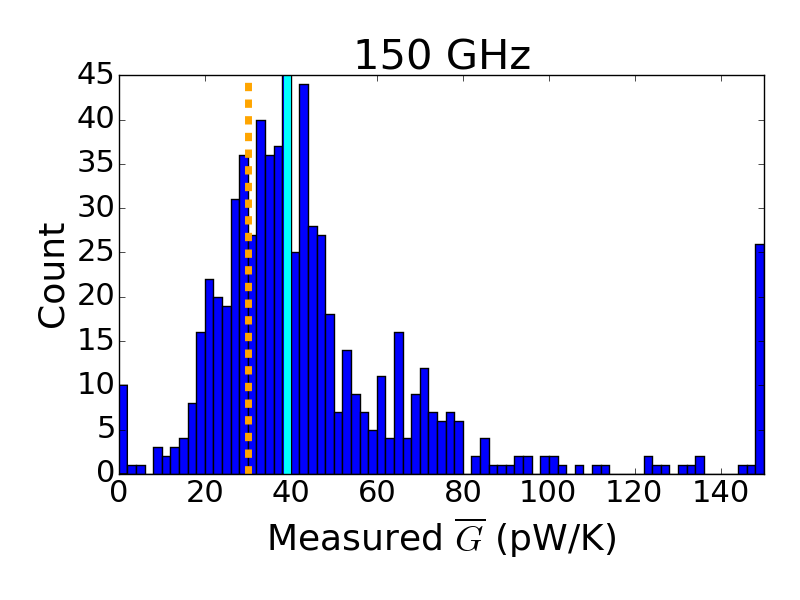
\includegraphics[width=0.32\columnwidth]{figures/150_g_bar_hist.png}
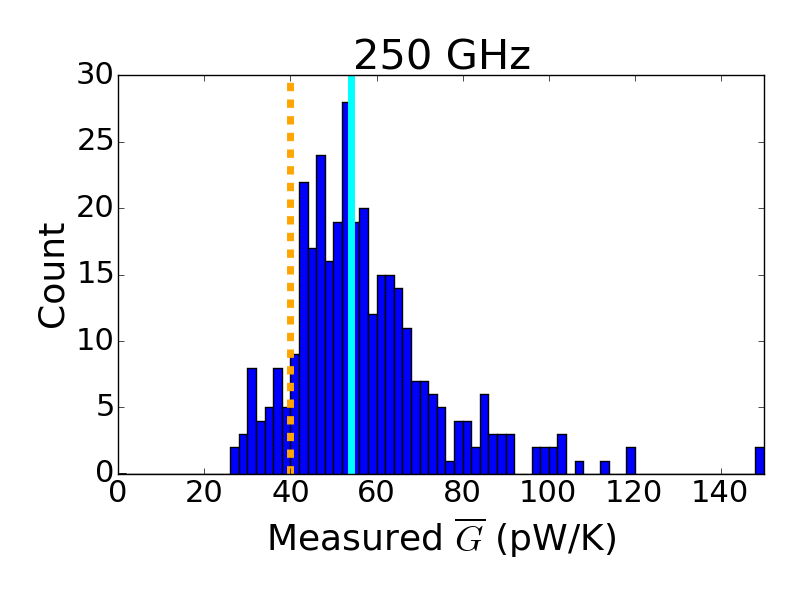
\includegraphics[width=0.32\columnwidth]{figures/250_g_bar_hist.png}
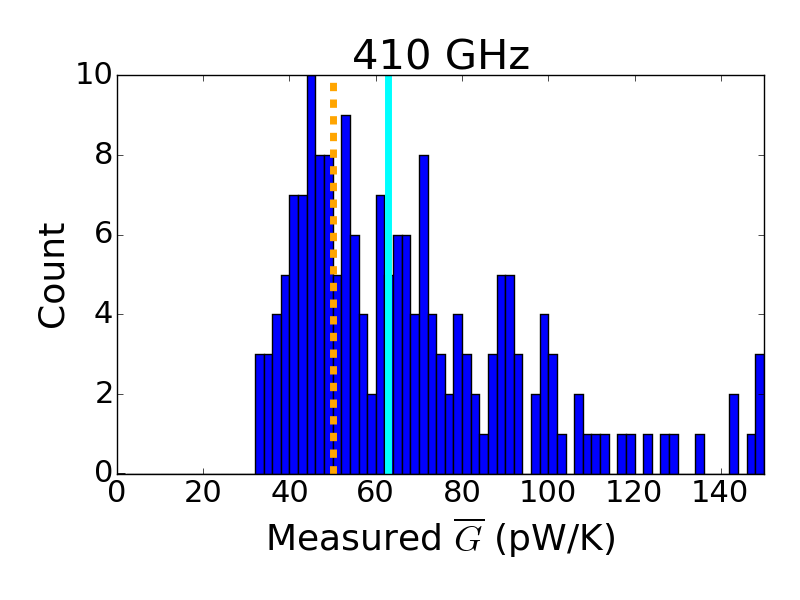
\includegraphics[width=0.32\columnwidth]{figures/410_g_bar_hist.png}
\caption{Histograms of the measured average thermal conductance values for the three frequency bands including the 
median (vertical cyan) and design (vertical gold dashed) values. 
We piled measurements of  $\overline{G}$ exceeding 150~pW/K into the last histogram bin.
}
\label{fig:G_Histograms} 
\end{figure}



%\textcolor{red}{This doesn't matter? You're not giving a play-by-play accounting.}
%Once the resonant frequencies are determined from the network analysis fits, the stage is heated so the bolometers are above their critical temperatures. 
%The bolometers are then electrically overbiased such that there is enough Joule Power dissipated in the \ac{TES} to keep its resistance normal as the stage is cooled. 
%Once the stage is at its base temperature, we measure the bolometer saturation powers. 


%FROM THE PAPER
%We determine the average thermal conductance of the bolometers using the relation
%\begin{equation}
% \overline{G}(T_{0}) = P_{sat}(T_0)/ (T_{c} - T_{0}),
%\label{eqn:gbar}
%\end{equation}
%where $P_{sat}$ is the total power deposited in the detector, which is the power necessary to operate the \ac{TES} in the regime of strong electrothermal feedback in which the total power absorbed is constant.
%This power is commonly called the `saturation power' and it depends on the temperature of the bath
%\begin{equation}
%P_{sat}(T_{0}) = P_{e} (T_{0}) + P_{abs}. 
%\label{eqn:boloPowerFlow}
%\end{equation}
%Here $P_{e}$ is the electrical power absorbed in Joule heating and $P_{abs}$ is the radiative power absorbed.
%In dark conditions we assume that $P_{abs}$~=~0, and so $P_{sat}(T_{0})$~=~$P_{e,d}(T_{0})$ is 
%therefore a measurable quantity; we added the subscript $_{d}$ to $P_{e,d}$ to highlight that this is the electrical 
%power measured in dark conditions. 

%FROM THE PAPER
%Histograms summarizing the measured average thermal conductance values for the three \ac{EBEX} frequency bands are shown in 
%Figure~\ref{fig:G_Histograms}. The values of  $\overline{G}$ are given for the \ac{EBEX} bath temperature, $T_{0}$~=~0.25~K.
%The measurements were conducted in three different cryostats, each operating at 
%a different bath temperature $T_{0'}$. We corrected the measured values $\overline{G}(T_{0'})$ to $\overline{G}(T_{0})$ using 
%the scaling
%\begin{equation}
%P_{sat}(T_0) = \left( \frac{T^{n+1}-T_0^{n+1}}{T^{n+1}-T_{0'}^{n+1}} \right) P_{sat}(T_{0'}),
%\label{eqn:ScalePsat}
%\end{equation}
%which assumes that the thermal conductivity follows a power law $\kappa$~=~$\kappa_{0} T^{n}$; see Section~\ref{sec:optical_time_constant}. 
%
%FROM THE PAPER
%The design and median of measured values for the average thermal conductances are given in Table~\ref{tab:Design_Params}. While the 
%measured medians are up to 40\% larger than the design values, the spread in the measurements is even larger. This spread is 
%a consequence of variance between wafers and is also apparent in the measurements of $T_{c}$. 
%Higher thermal conductance increases phonon noise. For example, for a median 410~GHz detector, phonon noise increased by 
%% for histograms using only flight bolos, median was 69
%%17\% relative to the nominal value of 26~$aW/\sqrt{Hz}$.
%% for histograms using all ground characterization data, median is 63. so percent decreased. 
%12\% relative to the nominal value of 26~$aW/\sqrt{\mathrm{Hz}}$. 



%%%%%%%%%%%%%%%%%%%%%%%%%%%%%%%%%%%%%%%%%%%%%%%%%%%%%%%%%%%%%%%%%%%%%%%%%%%%%%%%
\subsection{Optical Efficiency}
\label{sec:optical_efficiency}
%%%%%%%%%%%%%%%%%%%%%%%%%%%%%%%%%%%%%%%%%%%%%%%%%%%%%%%%%%%%%%%%%%%%%%%%%%%%%%%%

%\textcolor{red}{Oh, I wish you had time to remake the bb intensity versus frequency plot so you could actually read the axes.}
%
%\textcolor{red}{Remove labels that you don't use, e.g. SqCh1 Ch2. Also, if you don't use the resistance curve, do you want it in there?}

\textcolor{red}{Please include pictures or designs of the optics stack + blackbody. Or maybe the teflon mould or box lid, etc ?}

\textcolor{red}{At the very least, you need to explain that there was only a single hexagon of detectors open to the blackbody and they had their own EBEX optics stack.}

%\textcolor{red}{Re: Rederiving how black is blackbody (threw away the f-ing papers???). from cobe firas blackbody paper: "The optical properties of the Eccosorb have been report- ed (Hemmati, Mather, \& Eichhorn 1985; Peterson \& Richards 1984; Halpern et al. 1986)"}

\textcolor{red}{I want you to comment on the abosprtivity/reflectivity of eccosorb cr-110 as a function of frequency!}

In order to measure the optical efficiency of the \ac{EBEX} bolometers, the bolometers needed to observe a known, controllable radiative load.
This radiative load was provided via a blackbody, a body absorbing all incident radiation falling upon it. 
The \ac{ETC} blackbody was inspired by the design of Peterson and Richards for calibrating IR photometers \cite{Peterson1984a}. 
The blackbody itself was an inverted cone with an angle of 37$^{\circ}$, Figure~\ref{fig:blackbody_design}. 
The blackbody was made by pouring castable Eccosorb CR-110 into a teflon mould and baking it.
For mm-wave radiation incident on flat Eccosorb CR-110 at XXX~K, 30\% is reflected and 70\% refracted \cite{}.
%Eccosorb CR-110 reflects 30\% and refracts 70\% of radiation incident on its surface. %at XXX GHz.
The refracted radiation was absorbed inside the cone. 
The reflected radiation for the light ray with the outermost angle, the one with the fewest bounces,  
%(the \ac{EBEX} 150~GHz detectors had a field of view of 20$^{\circ}$) %already said in caption
reflected off the Eccosorb surface four times.
%, $0.3  4 = XXX$ absorptivity. 
Fewer than 8 parts in 1000 of the incident radiation escaped the blackbody. 
A steeper cone would have had greater absorptivity, but the height was limited by the dimensions of the \ac{ETC}. 

\begin{figure}[htp]
\begin{center}
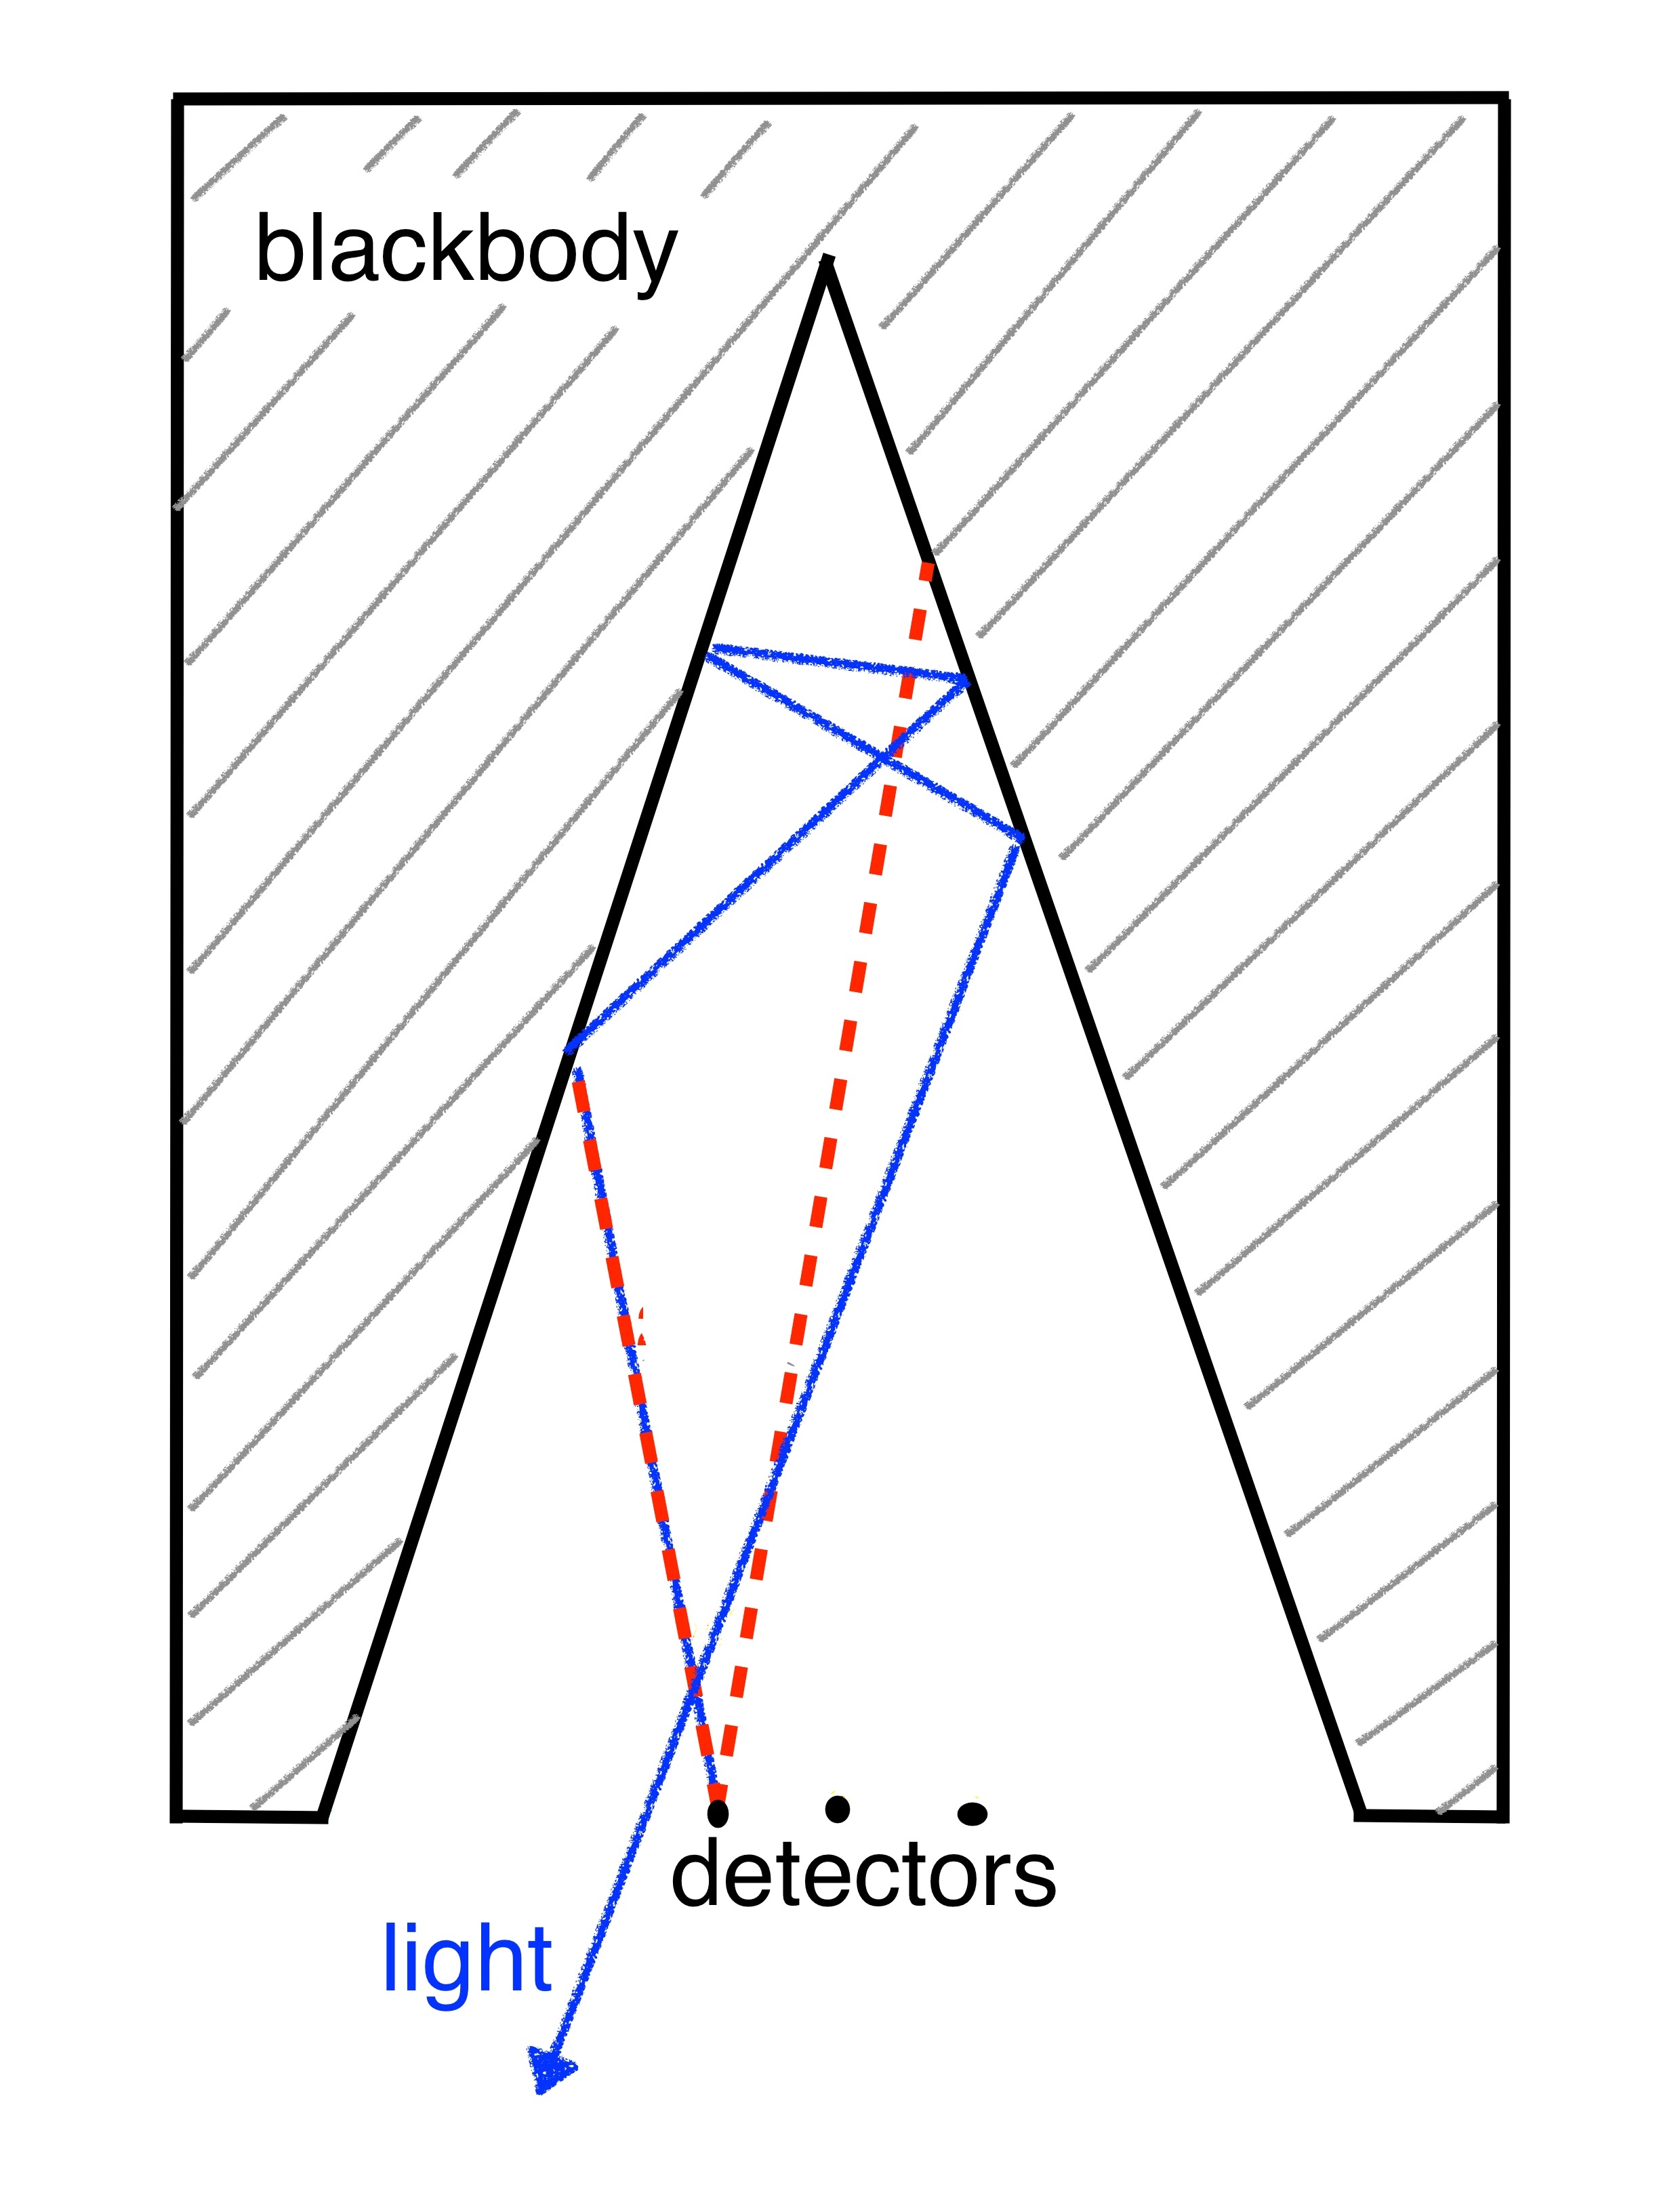
\includegraphics[height=2.5in]{figures/blackbody_design.jpeg}
\caption{Eccosorb blackbody design above detectors (black dots). The detector's field of view (red dashed lines) was 20$^{\circ}$. The blackbody cone had an opening angle of 37$^{\circ}$. The outermost light ray (blue line) bounced off the surface of the blackbody four times. 
\label{fig:blackbody_design} }
\end{center}
\end{figure}

A model of the optical efficiency testbed is shown in Figure~\ref{fig:opt_eff_setup}. 
The wafer box was supported by a thin (XXX) column of XXX. 
With the cold plate at a temperature of 4.2~K, the leg put a heat load of XXX on the fridge. 
The blackbody was supported by a thin column XXX. 
For the hexagon of seven detectors open to the blackbody, the wafer box had a miniature optics stack of wave guides and horns, to provide the high pass cutoff, and Cardiff LPE filter scraps, for the low pass cutoff. 


%ADD PICTURE IF YOU HAVE TIME
\begin{figure}[htp]
\begin{center}
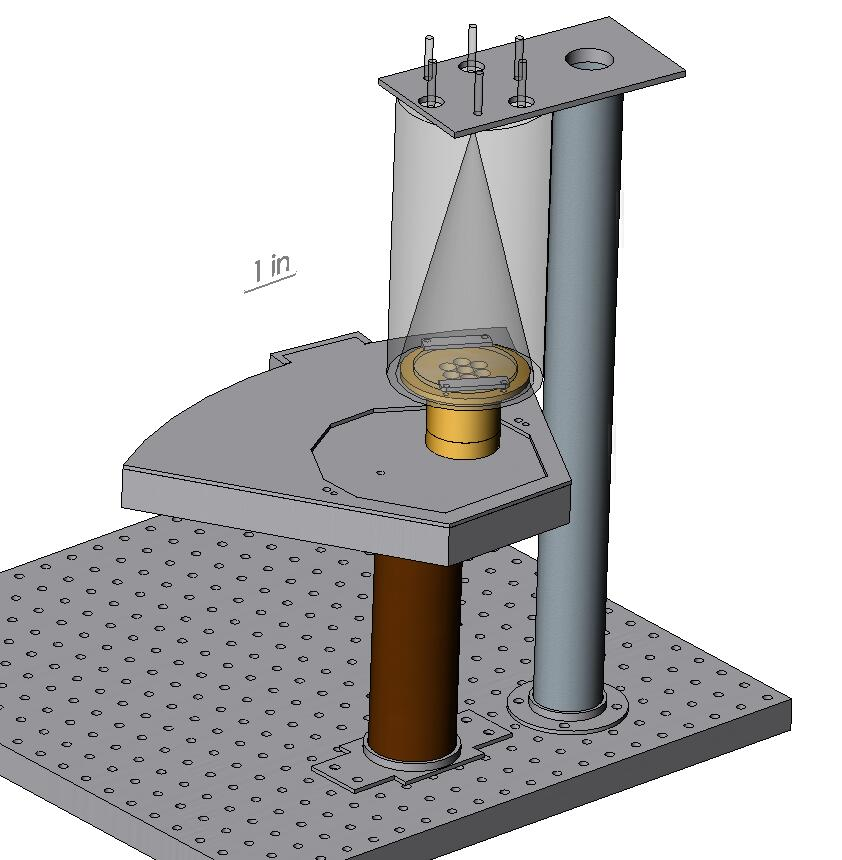
\includegraphics[height=2.5in]{figures/optical_efficiency_setup.jpg}
%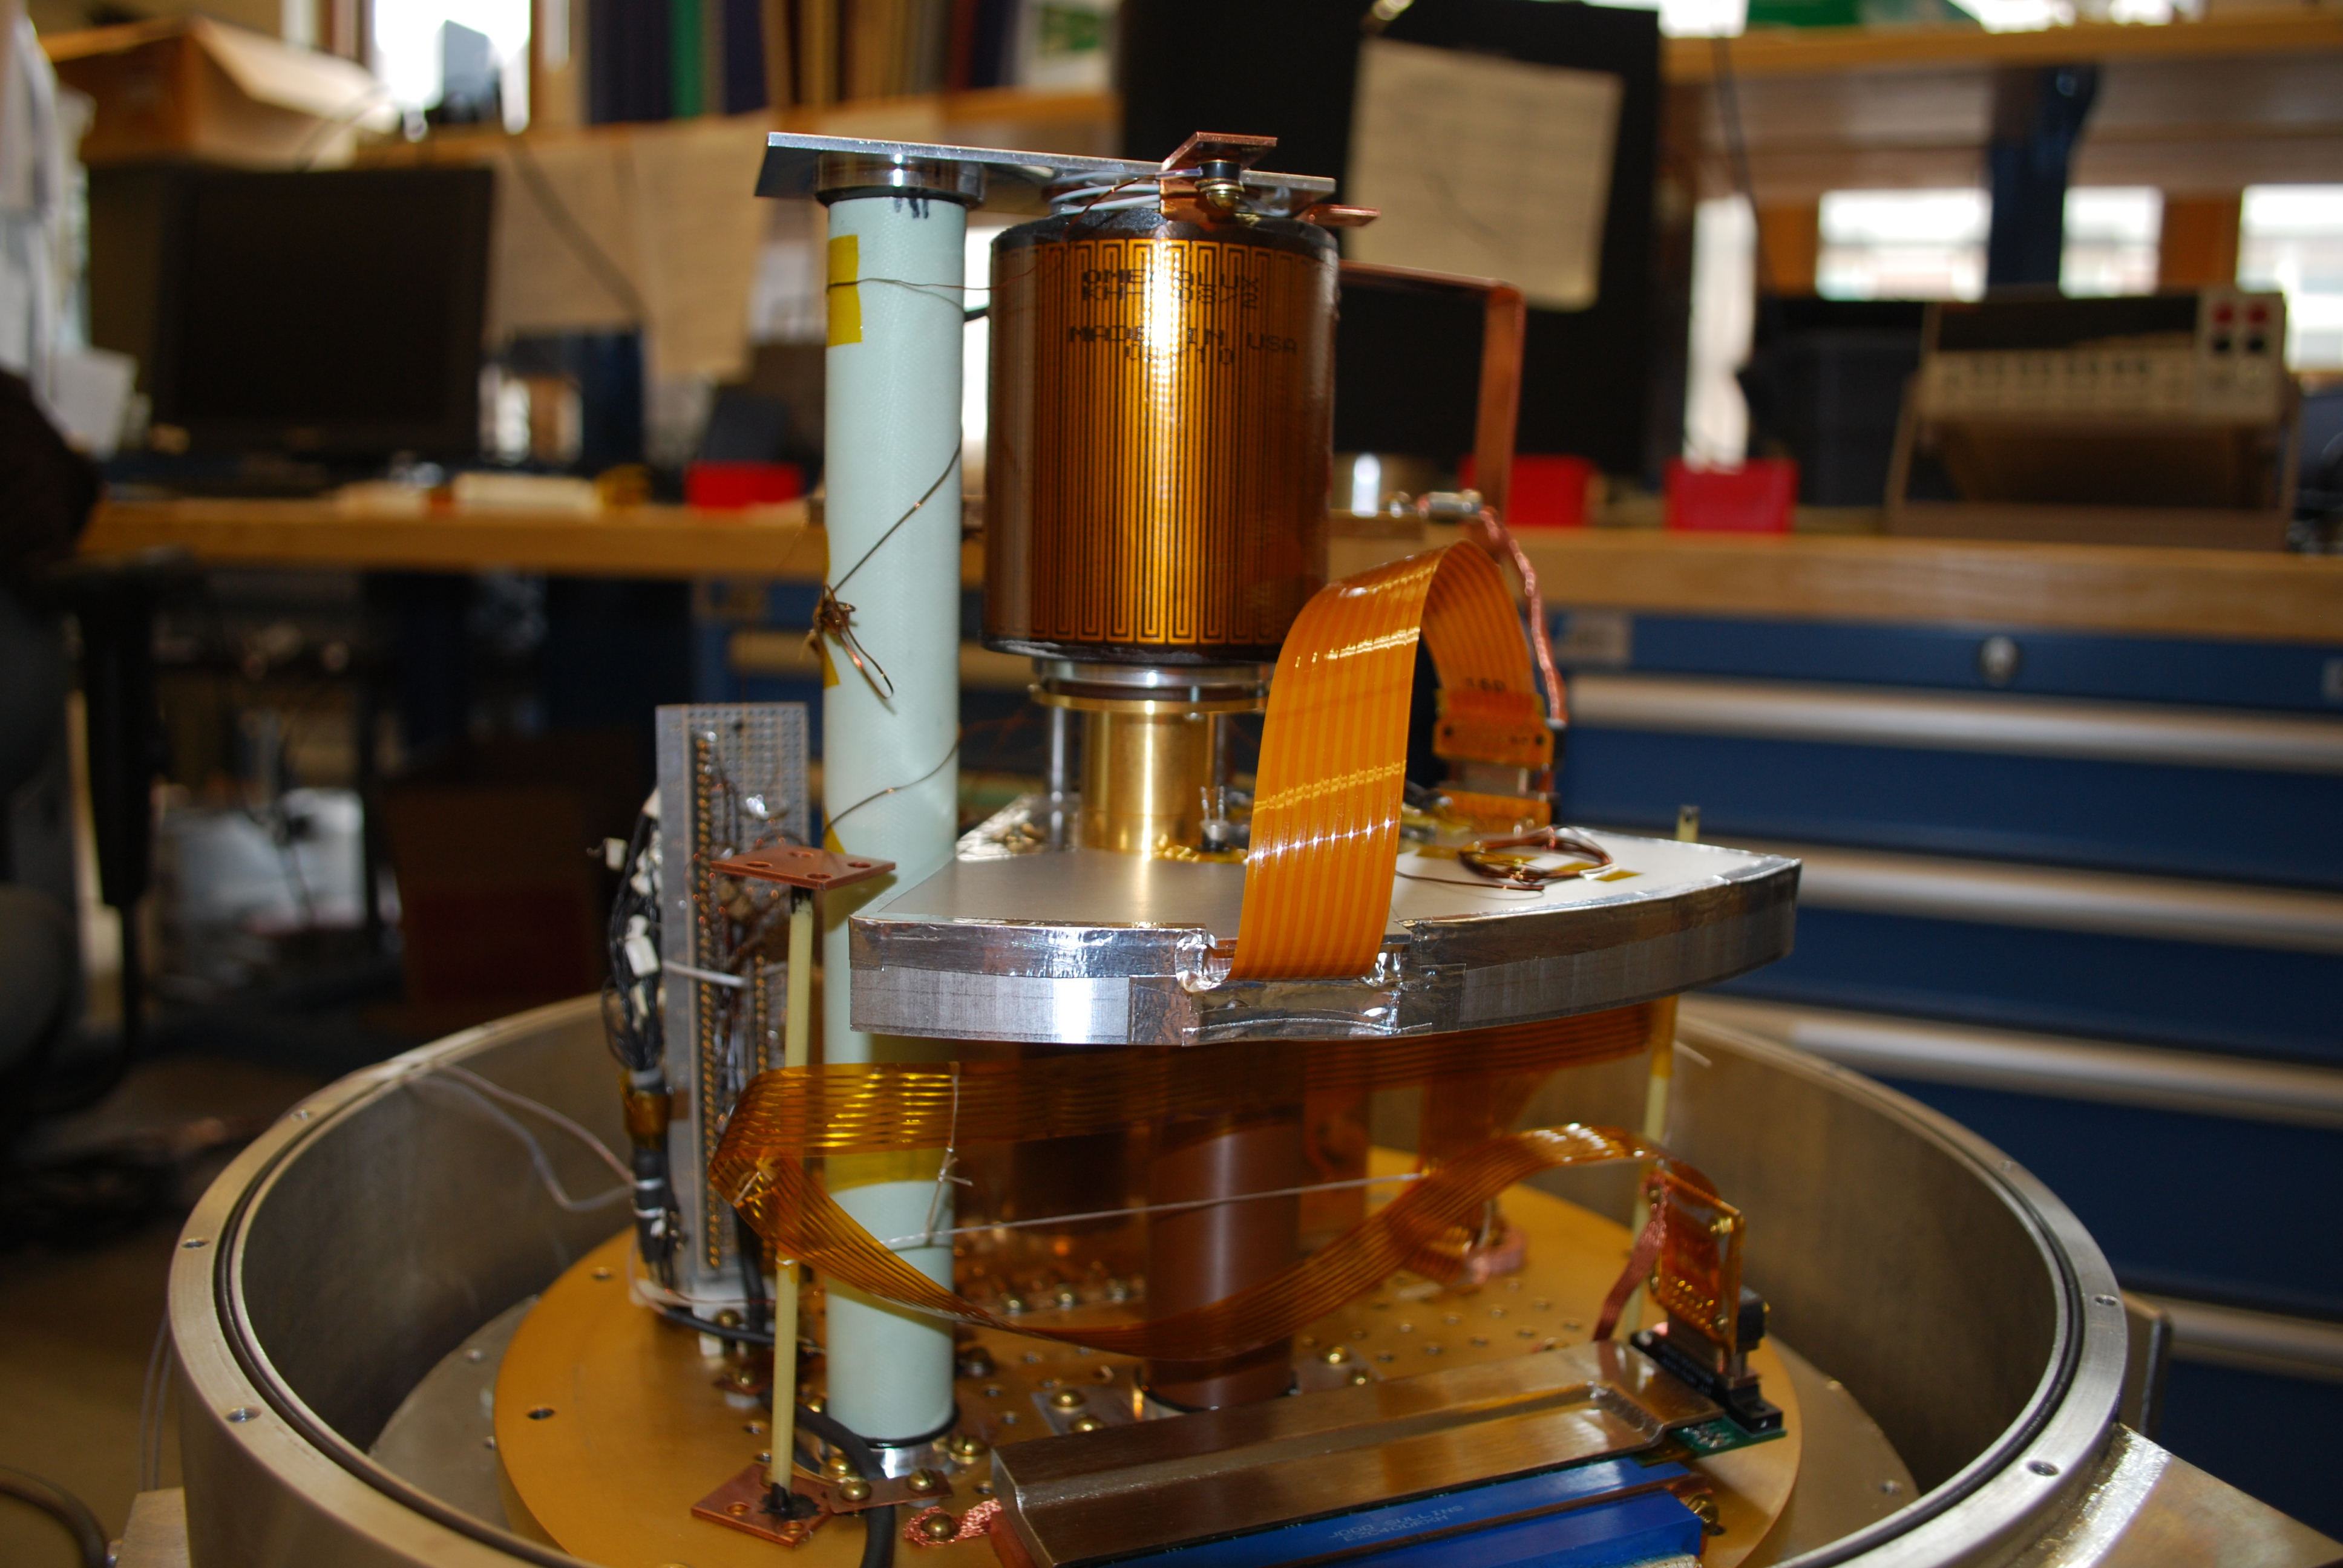
\includegraphics[width=0.48\columnwidth]{figures/hardware/opt_eff_setup_picture4.jpg}
\caption{The model of the optical efficiency testbed in \ac{ETC}. 
The blackbody is the partially transparent cone. 
The grey box atop the brown leg encloses the wafer 
The wafer box and blackbody are both mounted to the 4.2~K cold plate. 
%Right: \textcolor{red}{While it would be lovely to have a photograph of the setup, getting this to some understandable state is probably not something you have time for.}
\label{fig:opt_eff_setup} }
\end{center}
\end{figure}

There was a cooper bar embedded inside the Eccosorb for mounting a temperature sensor. %RuOx?
To cool the blackbody down from room temperature, a copper bar embedded in the Eccosorb was connected to the 4~K plate via a gas-gap heat switch.
For the optical efficiency measurements, the heat switch was opened and the blackbody temperature was controlled by a flat copper heater glued to the outside of the cone.


\begin{figure}[htp]
\begin{center}
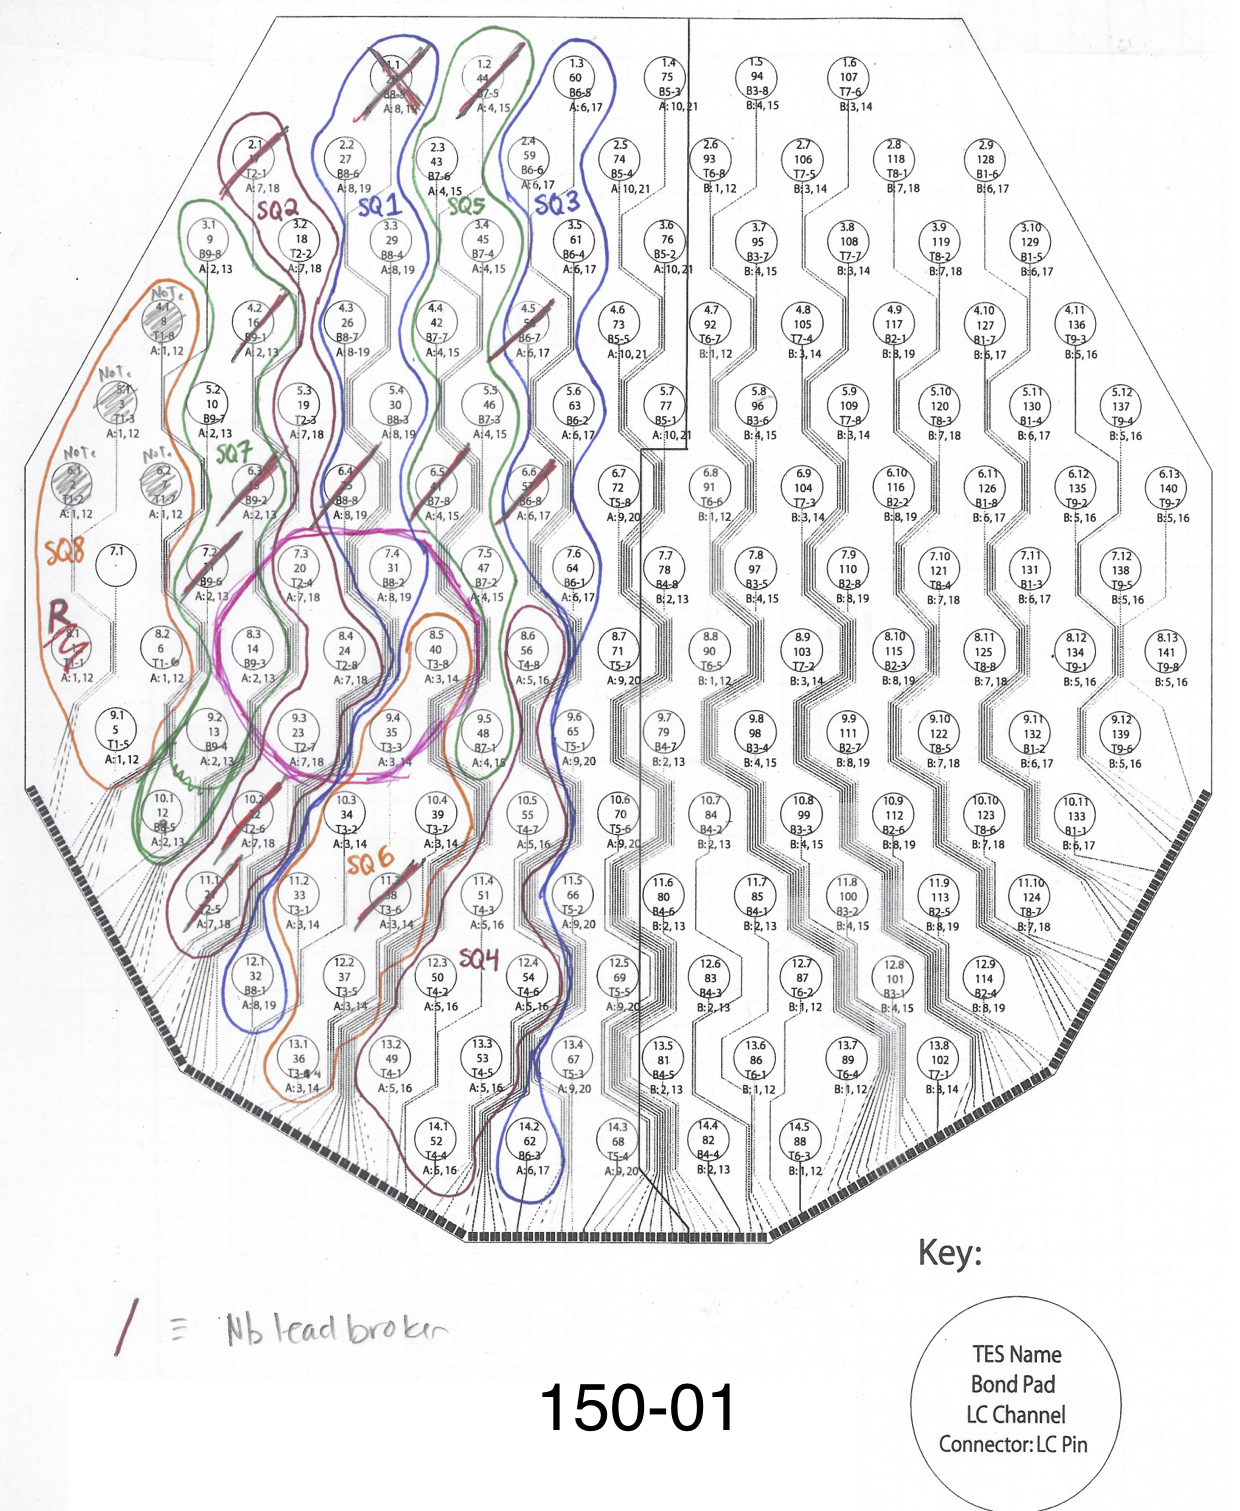
\includegraphics[height=7in]{figures/EBEX_Nb01_150GHz_wafer_schem.png}
\caption{Blackbody setup x8 multiplexing readout setup for wafer~150-01. Within the pink ring were the hexagon of detectors open to the blackbody. Squid groups were outlined in different colors and labelled SQ$N$, for $N \in (1,8)$. Non-functioning detectors were crossed out. 
\label{fig:bb_wafer_layout} }
\end{center}
\end{figure}


The x8 multiplexing readout schematic for wafer~150-01 with the blackbody setup is shown in Figure~\ref{fig:bb_wafer_layout}. 
Each detector was represented by a circle with several identifying labels (the bolometer's row-column name, the wire bonding pad number, the channel number on the \ac{LC} board, and the pin from the \ac{LC} board to the \ac{SQUID} board).
There was a hexagon of 7~bolometers (outlined in pink), with an optical stack of wave guides, cones, and miniature \ac{EBEX} low-pass radiative filters, open to the blackbody. 
%I WANT YOU TO REFERENCE A FIGURE OF THE MINI OPTICS STACK HERE!!
The other detectors were looking at the 320~mK box enclosing them. %wait, for the bb setup, was the box actually 320~mK?
The lines leading from each circle to the edge of the wafer were the bolometer's niobium leads to the wire bonding pads. 
The grouping of the bolometers read out by each \ac{SQUID} were indicated by outlines of different colors.
The non-functioning detectors were crossed off. 

As discussed in Section~\ref{}, the total power dissipated in the detector is
\begin{equation}
P = P_{elec} + \epsilon P_{rad} = \overline{G} \Delta T
\label{eq:bolo_power}
\end{equation}
where $\epsilon$ is the detector optical efficiency. 
For several temperatures of the blackbody, the electrical power required to hold the detector in the transition was measured, Figure~\ref{fig:opt_eff_bb_curves}.
As the blackbody temperature increased, the electrical power decreased.  
By 9~K, the power from the blackbody alone saturated the detectors. 
That is, there was no turnaround observed in the IV curve, the bolometer was normal even when the electrical power was at zero. 

\begin{figure}[htp]
\begin{center}
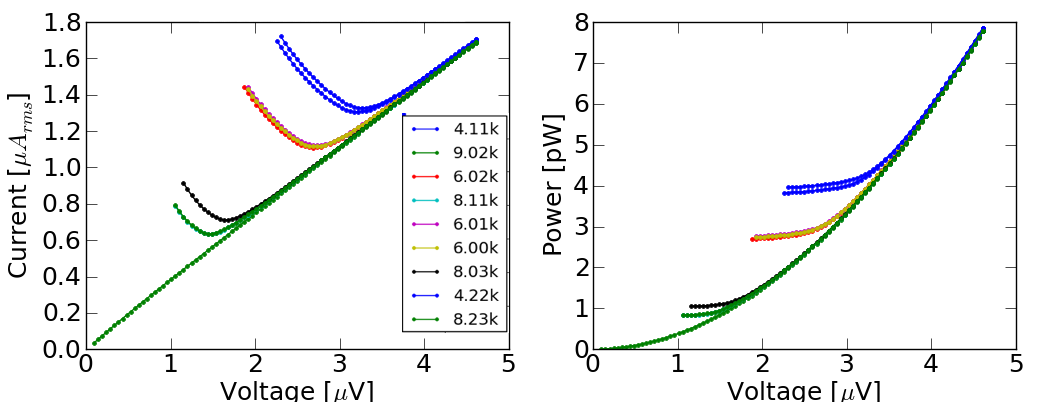
\includegraphics[height=2in]{figures/SqCh2_Ch1_all_bb_curves.png}
\caption{IV (left) and PV (right) curves for wafer 150-01 bolometer 8-04. The electrical power required to hold the detector in the transition decreases as the blackbody temperature increases. 
\label{fig:opt_eff_bb_curves} }
\end{center}
\end{figure}

The blackbody radiation curve was integrated over the \ac{EBEX} 150~GHz observation band to determine the amount of power incident upon the detectors at each blackbody temperature, left panel of Figure~\ref{fig:pelec_vs_popt}.
Rearranging Equation~\ref{eq:bolo_power}, we get the electrical power as a function of the radiative load
\begin{equation}
P_{elec} = \overline{G} \Delta T -  \epsilon P_{rad} 
\end{equation}
The slope of the line is the optical efficiency, $\epsilon$.
The right panel of Figure~\ref{fig:pelec_vs_popt} is the fit for wafer~150-01 bolometer~8-04. 
Table~\ref{tab:opt_eff} gives the slope for each of the functioning bolometers open to the blackbody. 

\begin{figure}[htp]
\begin{center}
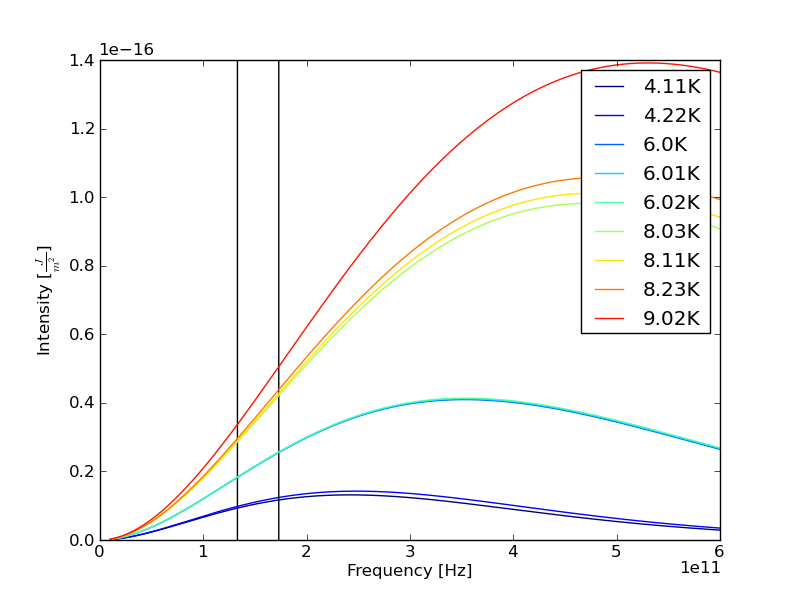
\includegraphics[width=0.49\columnwidth]{figures/blackbody_intensity_plot.png}
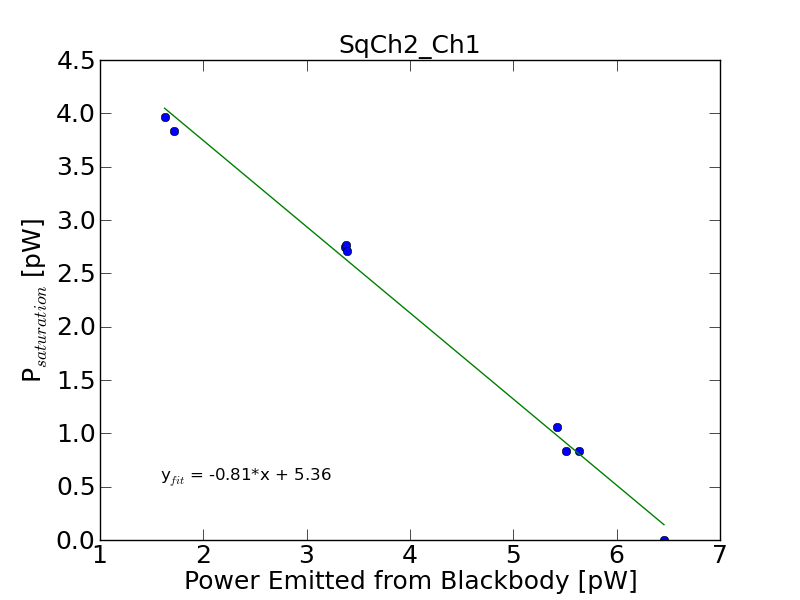
\includegraphics[width=0.48\columnwidth]{figures/SqCh2_Ch1_p_vs_p.png}
\caption{Left: Blackbody radiation as a function of temperature. The \ac{EBEX} 150~GHz band is marked by the black vertical lines. Right: Wafer~150-01 bolometer 8-04 electrical power as function of blackbody power. The slope, $\sim0.8$, is the detector's optical efficiency. 
%\textcolor{red}{remake this figure st the x-axis is labeled Prad not PBB!}
\label{fig:pelec_vs_popt} }
\end{center}
\end{figure}

\begin{table}[htp]
\begin{center}
\begin{tabular}{|c|c|}
bolometer & efficiency \\
7-03	& 66\% \\
7-04	& 87\% \\
8-03	& 74\% \\
8-04	& 81\% \\
9-03	& 74\% \\
\end{tabular}
\end{center}
\caption{Measured optical efficiencies of wafer~150-01 bolometers open to blackbody in \ac{ETC}.
\label{tab:opt_eff} }
\end{table}


\textcolor{red}{HERE you need to talk about:
\begin{itemize}
\item what is the uncertainty on the final percentage you quote? what are the major uncertainties in the optical efficiency measurement?
\item also note, the load the dark detectors saw. how big was it? why did they see it? what, if anything, does that say about the optical efficiency measurement for the detectors open to the blackbody? 
\item say if this is or is not consistent with other measurements of EBEX detector optical efficiency
\end{itemize}
 }


\begin{figure}[htp]
\begin{center}
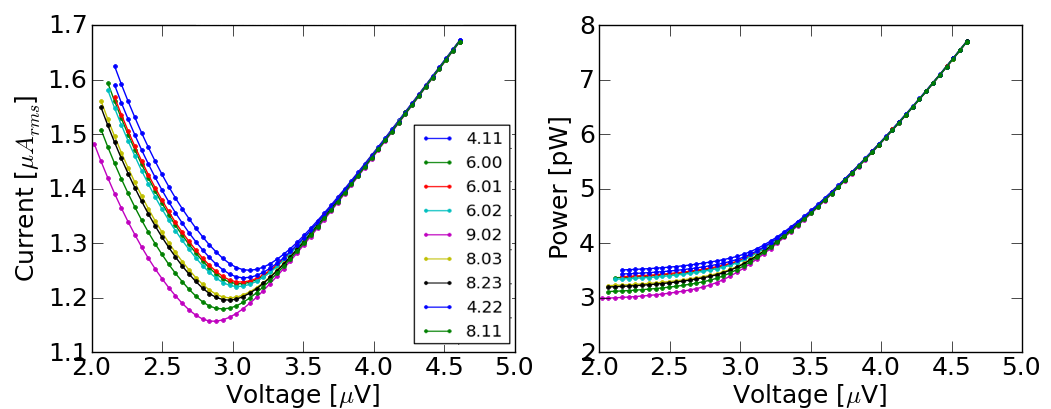
\includegraphics[width=0.65\columnwidth]{figures/SqCh7_Ch5_all_bb_curves.png}
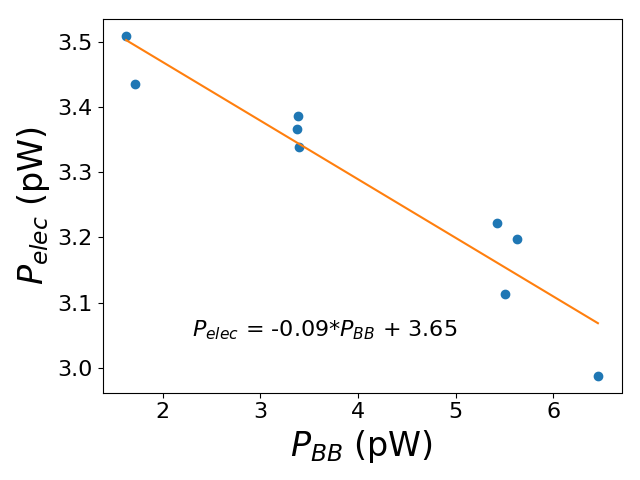
\includegraphics[width=0.33\columnwidth]{figures/SqCh7_Ch5_p_vs_p.png}
\caption{Left: Wafer~150-01 bolometer~10-01 IV curves as a function of blackbody temperature. Center: The PV curves for this same bolometer. Right: Though this detector was two rows away from the detectors open to the blackbody, the electrical power to hold the bolometer in its transition as a function of the black body power has a non-zero slope of $-0.09$. 
\label{fig:dark_pelec_vs_popt} }
\end{center}
\end{figure}


%
%\begin{figure}[ht!]
%\begin{center}
%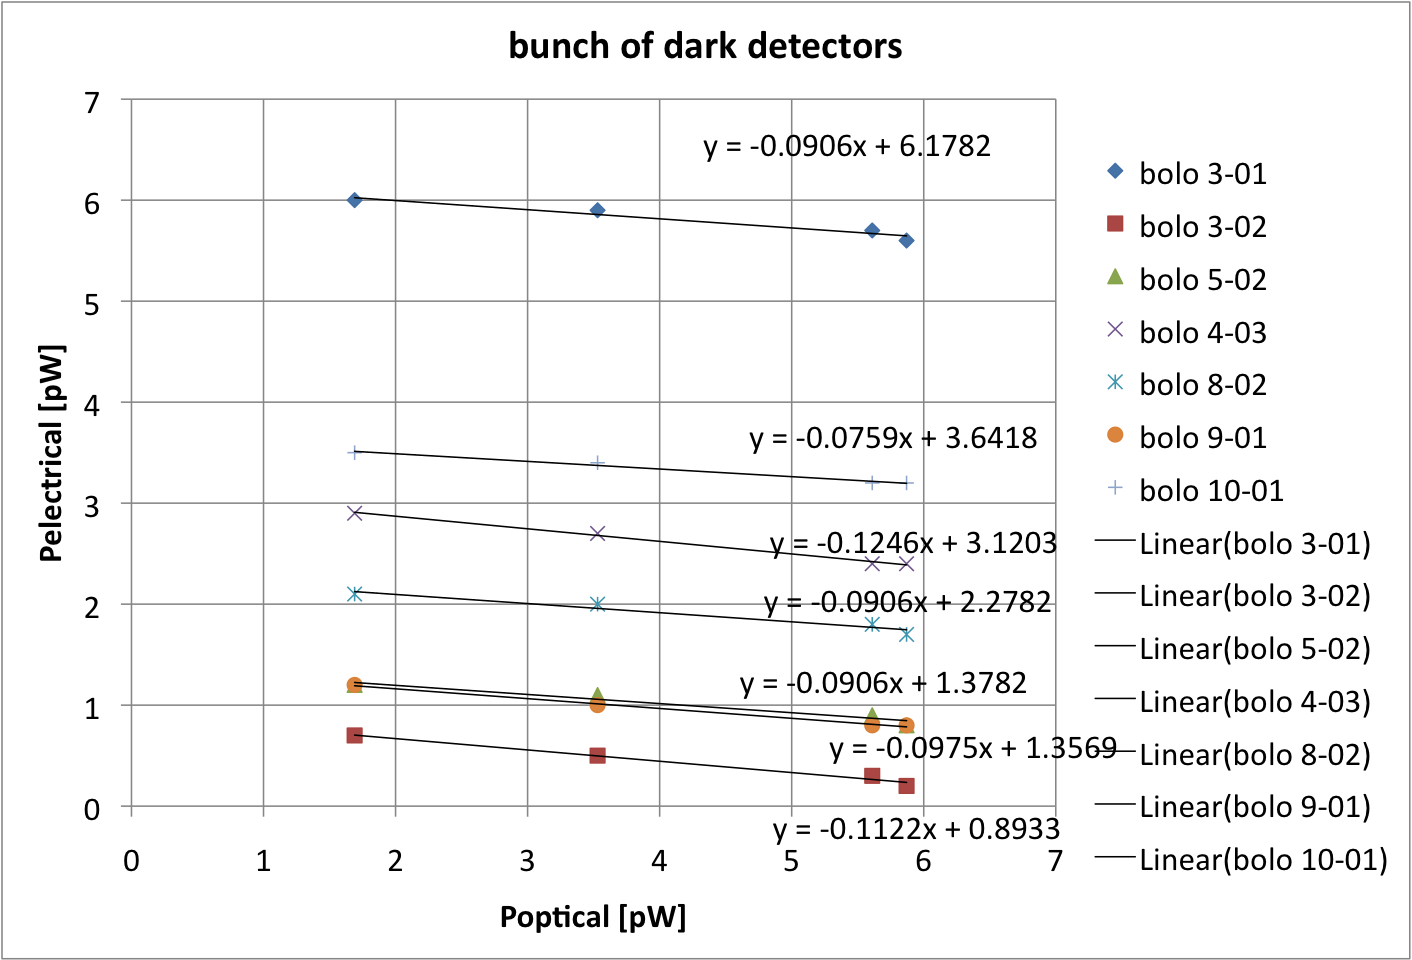
\includegraphics[height=2.5in]{figures/darkdetectoreffs}
%\caption{The dark detectors also observed a decrease in electrical power needed to keep the detector in the transition as the black body temperature was turned up. The slope of this line gives the "efficiency" of the dark detectors. Some measure of the level of optical cross talk?
%\label{fig:dark_optical_efficiencies} }
%\end{center}
%\end{figure}


%%%%%%%%%%%%%%%%%%%%%%%%%%%%%%%%%%%%%%%%%%%%%%%%%%%%%%%%%%%%%%%%%%%%%%%%%%%%%}}}

%%%%%%%%%%%%%%%%%%%%%%%%%%%%%%%%%%%%%%%%%%%%%%%%%%%%%%%%%%%%%%%%%%%%%%%%%%%%%%%%
\subsection{Time Constants}
\label{sec:time_constants}
%%%%%%%%%%%%%%%%%%%%%%%%%%%%%%%%%%%%%%%%%%%%%%%%%%%%%%%%%%%%%%%%%%%%%%%%%%%%%%%%

\textcolor{red}{Does this section get to make it in? We have electrothermal taus and IR taus ... Karl's fits were much more sophisticated. Can I include my stupid "fits"?}

\begin{figure}[ht!]
\begin{center}
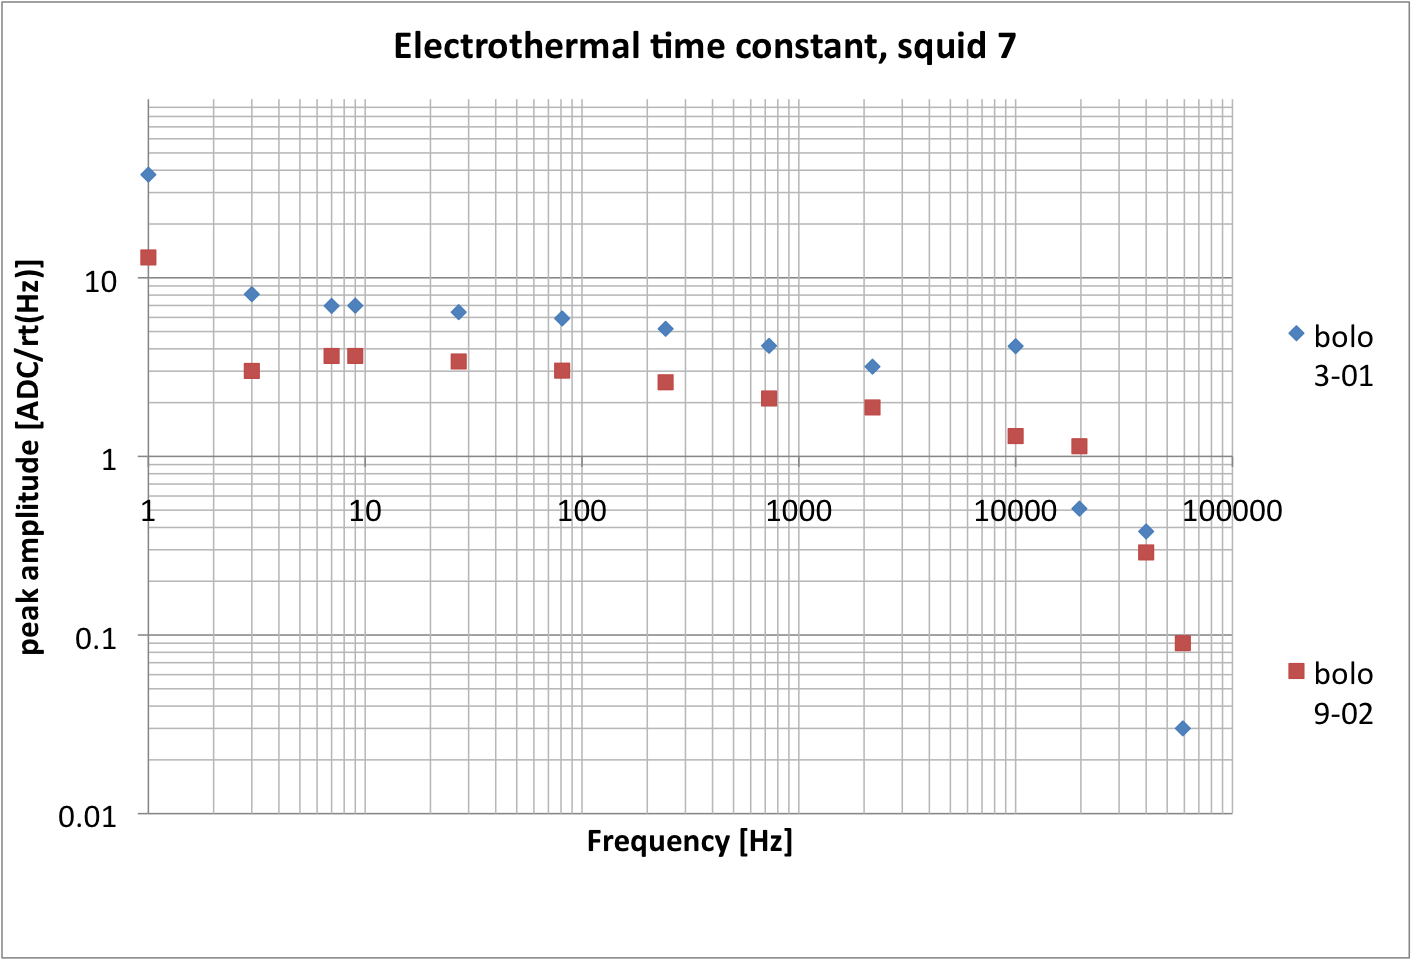
\includegraphics[width=0.48\columnwidth]{figures/Nb01_squid7_etau_morepts.png}
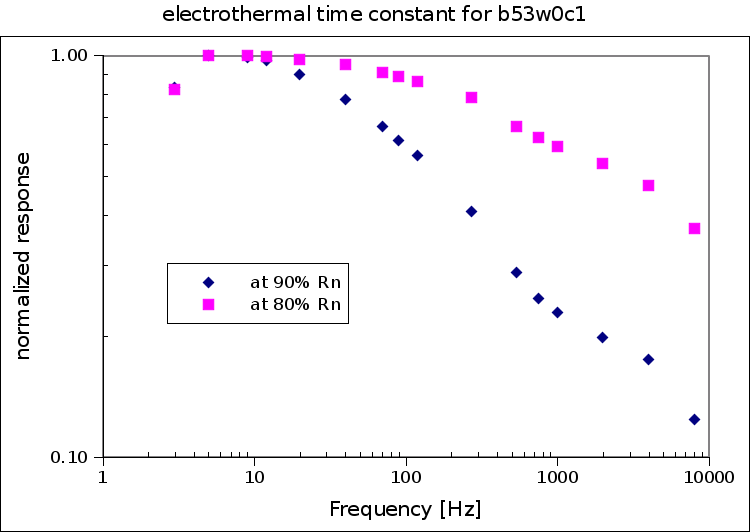
\includegraphics[width=0.48\columnwidth]{figures/b53w0c1_etau.png}
\caption{Left: Electrothermal time constants of two bolometers on 150-01. What does the fit to this data give? This is the time constant between the TES and the web? As expected, the for the web to thermalize is much faster than the optical time constant (time for light to couple to the web). Right: Electrothermal time constant for one bolometer on 150-02 at two depths in-transition ($0.9R_{initial}, 0.8R_{initial}$). 
\label{fig:electrothermal_tau} }
\end{center}
\end{figure}

\begin{figure}[ht!]
\begin{center}
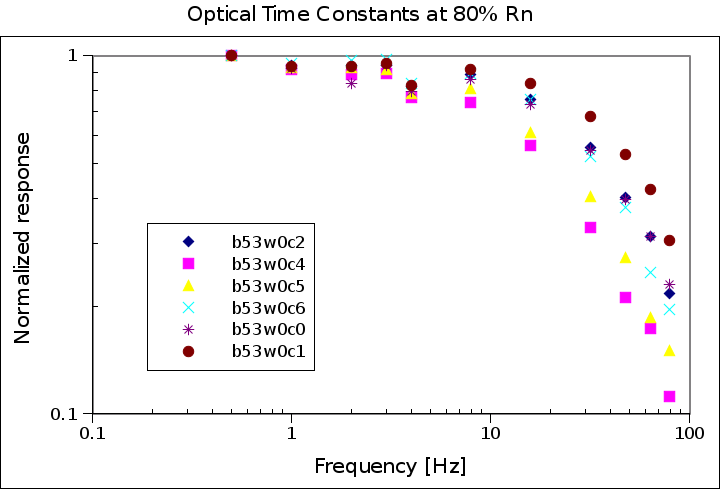
\includegraphics[height=2.5in]{figures/b53w0_ir_led_tau.png}
\caption{IR LED (Fairchild LED56) optical time constant measurement on 150-02. 
\label{fig:ir_led_tau} }
\end{center}
\end{figure}

\begin{table}[htp]
\caption{default}
\begin{center}
\begin{tabular}{|c|c|c|}
channel & frequency (Hz) & time constant (ms) \\
c0 & 18 & 8.8 \\
c1 & 30.5 & 5.2 \\
c2 & 20 & 8.0 \\
c4 & 10 & 15.9 \\
c5 & 10.5 & 15.2 \\
c6 & 19 & 8.4 \\
\end{tabular}
\end{center}
\caption{IR LED time constants for one comb of bolometers on 150-02, dark in \ac{ETC}. \textcolor{red}{What was the depth in transition?}
\label{tab:optical_tau} }
\end{table}







%%%%%%%%%%%%%%%%%%%%%%%%%%%%%%%%%%%%%%%%%%%%%%%%%%%%%%%%%%%%%%%%%%%%%%%%%%%%%}}}



%%%%%%%%%%%%%%%%%%%%%%%%%%%%%%%%%%%%%%%%%%%%%%%%%%%%%%%%%%%%%%%%%%%%%%%%%%%%%%%%
% Dark Noise Performance {{{
%%%%%%%%%%%%%%%%%%%%%%%%%%%%%%%%%%%%%%%%%%%%%%%%%%%%%%%%%%%%%%%%%%%%%%%%%%%%%%%%
\section{Dark Noise Performance}
\label{sec:dark_noise}
%%%%%%%%%%%%%%%%%%%%%%%%%%%%%%%%%%%%%%%%%%%%%%%%%%%%%%%%%%%%%%%%%%%%%%%%%%%%%%%%

%what is this section about
In order to understand the noise performance of each part of the detector readout chain, the noise measurements were broken down into 
room temperature electronics noise, 
electronics noise up to and including the 4~K \ac{SQUID}s, 
%the noise of resistor channels (i.e. the entire electronics chain up to the bond pads on the \ac{LC} board), %leave these out for now?! time...
the noise of the bolometers over-biased with the stage above the bolometers' $T_{c}$, 
the noise of the bolometers overbiased with the stage at the refrigerator's base temperature, 
and the noise of the bolometers in-transition as a function of their transition depth. 
The dark \ac{ETC} had the exact same electronics boards, filters, and cables as \ac{EBEX}. 
In \ac{ETC}, most of the measured noise agreed with the predictions until the bolometers were dropped below 90\% of their initial resistance. 

%attempting to explain method for measuring noise
For each noise measurement, $\sim3$ minutes of data was taken. 
We demodulated, \ac{ADC} counts were measured on the  \ac{DfMUX} board. 
We converted to nV or pA or aW. 
We calculated the PSD (pA2/Hz) and averaged from 0.5 to 5.0~Hz and then took the square root and called that the white noise level. 
Figure~\ref{fig:timestream_and_psd} is an example of a raw bolometer timestream converted to A for wafer~150-01 bolometer~3-01 as a function of sample number (there were 20MHz/2**17 (FIR stage) = 190.73 samples per second) and the corresponding PSD.

\begin{figure}[ht!]
\begin{center}
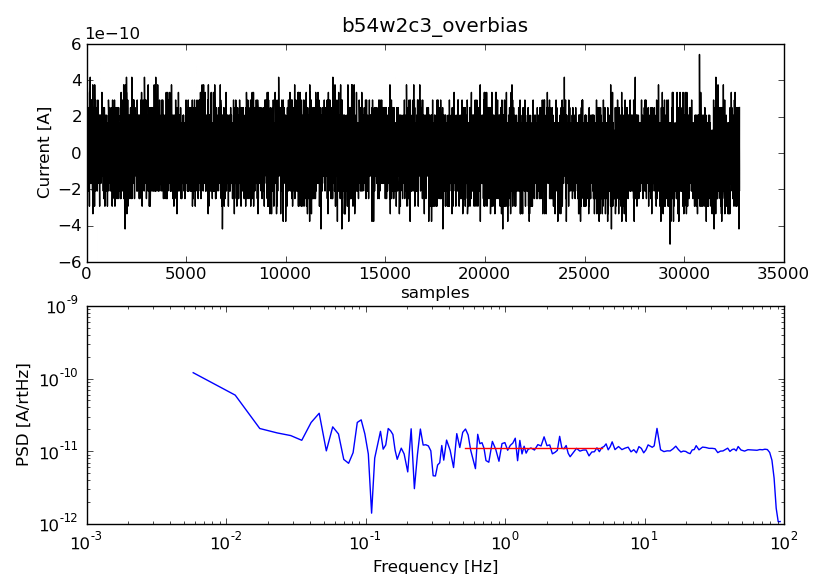
\includegraphics[height=2.5in]{figures/b54w2c3_overbias.png}
\caption{The raw bolometer timestream converted from \ac{ADC} counts to current and the PSD of that timestream for 150-01 bolometer 3-01 noise determination. The timestream was $\sim3$ minutes long. The white noise level was averaged from 0.5 to 5~Hz and for this bolometer had a value of 11.2 pA.
\label{fig:timestream_and_psd} }
\end{center}
\end{figure}



\textcolor{red}{You haven't shown any resistor noise!! How much of an investment in time is it to go back and reanalyze this? Is it sufficient to compare to the resistor analysis you did on the ground in the high bay? Doesn't really flow with your ETC story :/}

\textcolor{red}{can you draw a circuit diagram of the warm electronic noise you're measuring?}

%\textcolor{red}{Which electronic component is responsible for the roll off? It is the squid controller first stage amplifier. Can you get the specs to determine what roll off we expected? Can't find on wiki. Ask Franky. Then, answer, is it consistent with what we measured?}

\textcolor{red}{do you understand why we don't have this roll off when it's operating under normal conditions and why we DO have this roll off when it's open loop?}

\textcolor{red}{Is this $V_{rms}$ or $V_{p}$ ?}

\textcolor{red}{As you talk about noise, you need to be clear somewhere that you're using NEP and noise and ASD and PSD interchangeably. OR. don't use them interchangeably!}

%\textcolor{red}{Are you sure you have the contribution calculations correct? What are those $\sqrt{2}$s coming from??}

\textcolor{red}{If you're going to mention the 20 ohm resistor noise as a main contributor, you need to be able to point to where this is. perhaps say it in words and refer to Franky's thesis??}

%\textcolor{red}{before you dive in to plots where you have the white noise level/asd plotted on the y-axis, you need to describe how you obtained those data points!}

\textcolor{red}{Can you please be more specific about exactly which electronic components are included in this measurement?}

\textcolor{red}{Is there an apparent paradox here? You are measuring the warm electronic noise with the squids off, open loop. and you say the largest contributors are the 1st stage amplifier and the 20 ohm resistor. AND, you say those two noise contributions are the only reason you need the squid transimpedance. you're missing a key connection... when you close the feedback loop, then dv/di matters??? and when it's open, the noise prediction changes??}

\textcolor{red}{It's confusing to say the squids are off and then to say you've measured the noise for two squids ... word this better if you have time!}

\textcolor{red}{link to data sheet for texas instruments op amp 847 has open loop gain plot: http://www.ti.com/lit/ds/symlink/opa847.pdf    how do we even reference this??}

\textcolor{red}{Do you want to mention that in EBEX the transimpedance of the SQUIDs was higher (because they were a little colder ?)?}

\textcolor{red}{Do you want to make it clear that we measured squid noise in EBEX with dark squids not attached to any bolometers but in ETC we used squids attached to bolometers and just looked off resonance?}

\textcolor{red}{Figure out how to reference Franky's thesis and be sure you're doing it in all the right places. Also, is there some dfmux paper we should also be referencing?}

warm electronic noise open loop (with the squids off)
With the \ac{SQUID}s off, we measured the open loop noise.
%(no current bias, no flux bias, and no voltage offset) % no need to define off ... also, that's the voltage offset of ... the firs stage amplifier???
This was a measure of the noise of the warm electronics referred back to the input of the \ac{SQUID} controller first stage amplifier. 
The theoretical open loop transfer function was 0.774 nV to 1 \ac{ADC} count. 
The measured transfer function was a factor of 1.13 greater than the theoretical. 
Figure~\ref{fig:dark_electronic_noise} is the measured open loop warm electronics noise for two \ac{SQUID}s in \ac{ETC} as a function of the demodulation frequency. 
The total noise prediction was $1.33~nV/\sqrt{Hz}$, determined from the electronic specifications~\cite{Francois2012}. 
The largest contributors were the first stage amplifier of the \ac{SQUID} controller board, $0.85~nV/\sqrt{Hz}$, and that amplifier's $20~\Omega$ gain defining resistor Johnson noise, $0.57~nV/\sqrt{Hz}$. 
The measurement agrees with the prediction at low frequencies and then the signal rolls off, with a -3dB point around 1~MHz, because the first stage amplifier is being operated in the open-loop regime~\ref{data_sheet?}.  


\begin{figure}[ht!]
\begin{center}
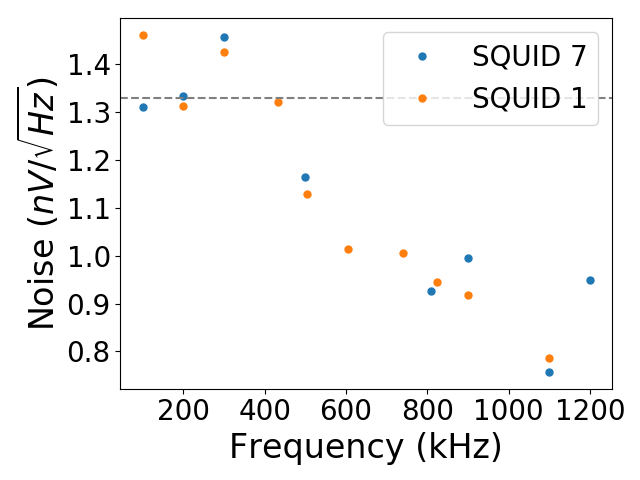
\includegraphics[height=2.5in]{figures/warm_electronic_noise.png}
\caption{Measured noise of the warm electronics in \ac{ETC} up to the first stage amplifier on the \ac{SQUID} controller board. The open loop noise at low frequencies was predicted to be 1.33~$nV/\sqrt{Hz}$ and to roll off with a -3dB point around 1~MHz. 
\label{fig:dark_electronic_noise} }
\end{center}
\end{figure}


\textcolor{red}{Are you at all interested in recording, for posterity's sake?, how you converted from $V_{DAC}$ to physical units in \ac{ETC}?? i.e. for the \ac{ETC} \ac{SQUID} controller board, $1 V_{DAC} = 1 mV$ and $1 V_{DAC} = 20 \mu A$ and mention mutual inductance $\phi_{0}/26 \mu A$?}

\textcolor{red}{do you want to mention what transimpedances we measured with the ebex squids?}

\textcolor{red}{ do you want to say HOW the value of $Z_{t} = dV/dI$ affects the noise predictions for the first stage amp and the 20ohm R?}

\textcolor{red}{How/why on earth did we estimate $\mathscr{L}_{FLL}$ to be 13? How did we even generate the plot of squid 7 loop gain vs demodulation frequency? that plot tells us it's a pretty dramatic function of frequency? Is there any reason taking the lower limit would be ok? In EBEX, we used the 5K feedback resistors?}

squids (with their feedback loops closed)
With the \ac{SQUID}s on and their feedback loops closed, the warm electronic components' noise predictions were referred to current noise at the \ac{SQUID} input coil.
The \ac{SQUID} transimpedance, $dV/dI$, was used to reference the noise of the \ac{SQUID} controller first stage amplifier and its gain defining 20~$\Omega$ resistor. 
We measured $dV/dI$ from the slope of the linear regime of the $V-\phi$ curve where we biased the squid, Figure~\ref{fig:squid_transimpedance}. 
The fit to the line in the region where this particular \ac{SQUID} from \ac{ETC} was biased gives a transimpedance of $dV/dI=375~\Omega$. 
The \ac{SQUID} flux-locked loop gain transfer function, $|\frac{(1-\mathscr{L}_{FLL})}{\mathscr{L}_{FLL}}|/R_{feedback}$ was used to reference the noise for those components after the first stage amplifier. 
The ampifier's feedback resistor value was known, typically $5~k\Omega$ or $10~k\Omega$, and the flux-locked loop gain, $\mathscr{L}_{FLL}$, was estimated to be 13, Figure~\ref{fig:squid_flux_locked_loopgain}. 

\begin{figure}[ht!]
\begin{center}
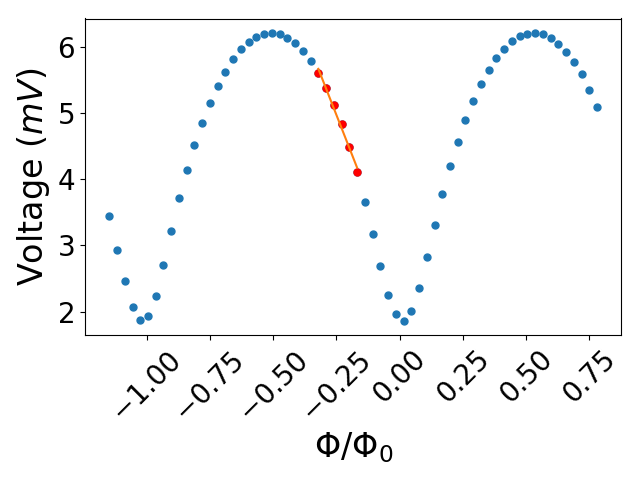
\includegraphics[height=2.5in]{figures/vphi_physical.png}
\caption{\ac{SQUID} voltage versus flux curve. The operating regime is highlighted (red) and fit to a line (orange) to get the \ac{SQUID} transimpedance.
\label{fig:squid_transimpedance} }
\end{center}
\end{figure}

%maybe better to just remove this plot? since you don't remember how you got it? 
%and, just take the value from hannes' thesis of Lfluxlockedloop = 13 for 10K feedback, even though it's clearly a strong function of frequency...

%\begin{figure}[ht!]
%\begin{center}
%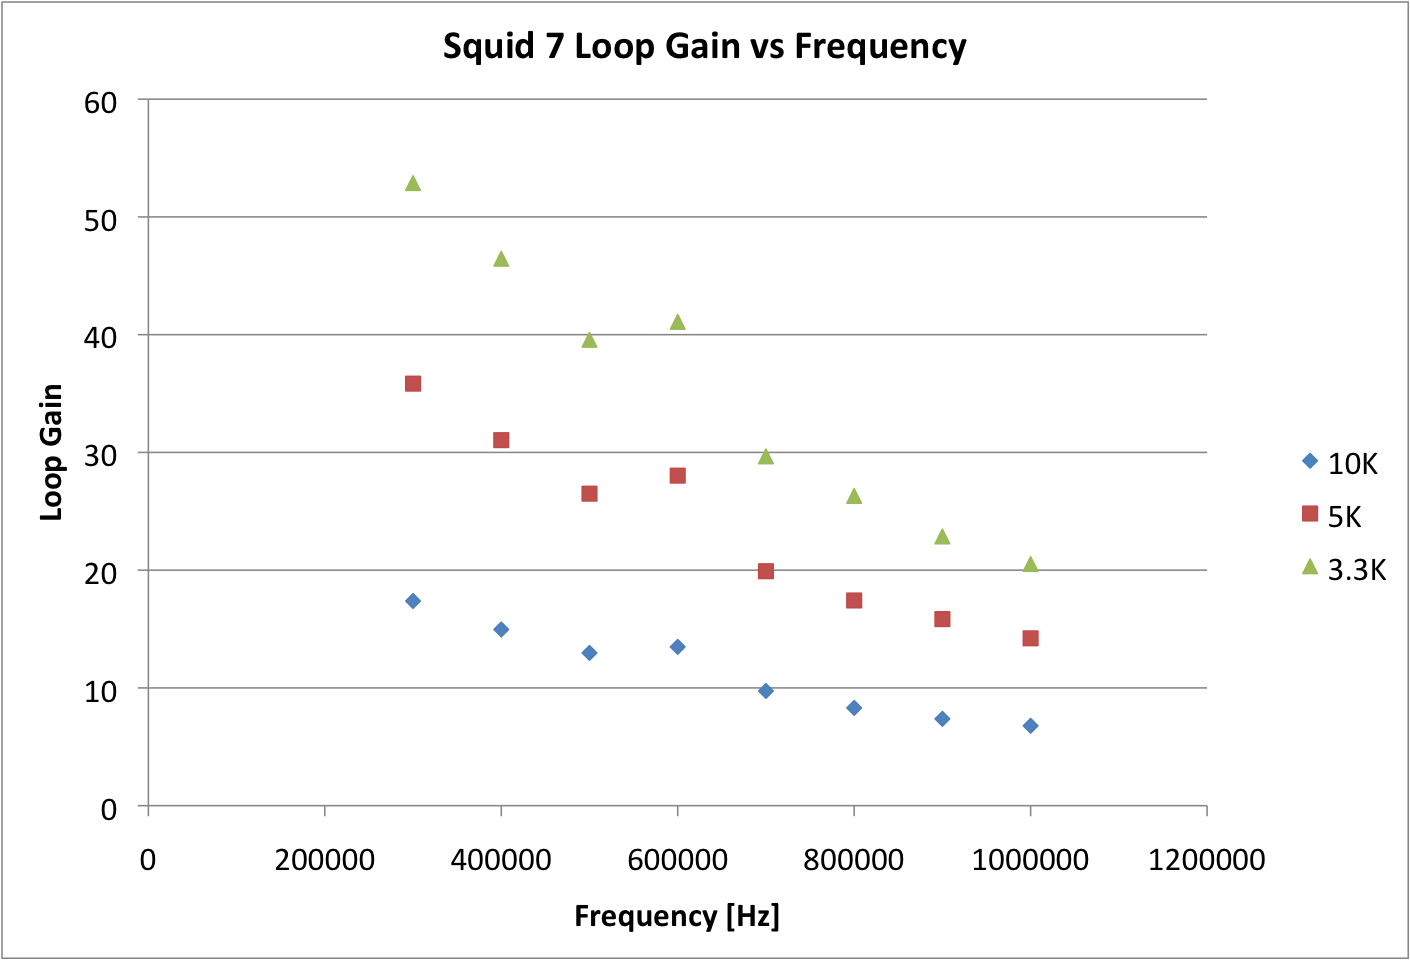
\includegraphics[height=2.5in]{figures/squid7_loopgain.png}
%\caption{We measured the \ac{SQUID} flux-locked loop gain. we did voltage (?) open loop over voltage (?) at Rfeedback -1. as a function of frequency. ???
%\label{fig:squid_flux_locked_loopgain} }
%\end{center}
%\end{figure}

\textcolor{red}{Include squid noise measured in EBEX at float in thesis? Later on in performance section? don't even mention here?}
%\textcolor{red}{These predictions are from an era where the squid noise was 2.5 pA/rtHz. Later on in this 150-01 run is where we adjusted the prediction to measure the measurement and found the intrinsic squid noise was more like 4pA/rtHz (though franky used 3.5 pA/rtHz in the analysis code). So. You should: 
%1. Include the plot of 2.5 and 4.0 pA/rtHz and explain why we changed the intrinsic noise "prediction" to match the measurement. 
%2. Adjust the predictions of the squid noise to reflect this. Perhaps just remake them? but how do I know what the dfmux board settings were? find the date and hope the settings are there? or calculate the noise with 2.5 and subtract it (in quadrature) and add the noise with 4.0? }

\textcolor{red}{Why is the on resonance noise higher than predicted? Do you want to find and include the 700mK squid noise data to say we don't know what's going on at 4.2~K, but meas/pred agree more at lower temperatures?}

\textcolor{red}{Is it appropriate to reference the conversation with the nist folks? you don't even remember when it was. should we simply not mention they thought that was reasonable? should we point to the paper where it said 2.5 pA/rtHz and say this was unreasonably low? from Huber et al the SQUID white noise level at 4.2K is 2.5 pArms/rtHz.}

\textcolor{red}{how can you say, at 4.2K, the predictions, for reasons we don't understand, seemed to put a lower limit on the measured Johnson noise. ?}

\textcolor{red}{and at 770 mK, we don't understand at all why the higher frequency demodulated noise is too high. What is the point of including the 770mK squid noise graph? That we don't understand what happens when we get cold? are you certain there were no carriers or nullers on for this measurement?}

\textcolor{red}{Are you going to mention 1. that you are including two squids (one and seven) and 2. why you are only including two squids?}

\textcolor{red}{I wanted to put labels indicating the temperature of the two squid noise plots, but I'm having troubles. So. Move on for now.}

\textcolor{red}{Do you want to zoom in on the in-transition noise up to, say R=0.6Rinitial? So the information isn't completely washed out by the gigantic noise very deep in the transition? If so, do you want this to be a sub panel of the noise plot? And just delete the legend?}

\textcolor{red}{Re: high noise in ETC for 150-01. You have the data for photon noise if you have a 4K blackbody (1.8 pW) and you could show how the prediction changes if ALL of this power is absorbed by the (dark) detectors. Still doesn't explain excess.}

\textcolor{red}{I want to generate a plot with more data for fracRn between 1 and 0.7 ... Do we have such a thing?}

\textcolor{red}{Do we have other noise data you can put together reasonably efficiently?}

\textcolor{red}{If we want, we can re-make plots of electrothermal time constants. And say they're sufficiently long so the optical time constant can dominate.}

\textcolor{red}{We can show a measure of the flux locked loopgain as a function of demodulation frequency. This informs some electronics noise terms (by Lfll - 1 / Lfll, or something like that).} 

%The \ac{SQUID} noise could be measured, as was done in \ac{EBEX}, on a \ac{SQUID} not attached to a comb of bolometers (typically because of an open on one end of the microstrip) or it could be measured, as was done in \ac{ETC}, on a \ac{SQUID} with bolometers attached, but demodulating away from their resonant frequencies. 
With the detectors at a temperature of 4.2~K, and without providing carrier or nuller biases, we measured the noise as a function of demodulation frequency, Figure~\ref{fig:dark_squid_noise}. 
Away from the bolometer resonant frequencies, this is a measure of the noise due to the warm electronics and the \ac{SQUID}s, Figure~\ref{fig:adjust_squid}. 
Earlier generations of this \ac{SQUID} design were reported to have a noise of 2.5~$pA/\sqrt{Hz}$, \cite{Huber2001}.
Since the warm electronic noise agreed with predictions, Figure~\ref{fig:dark_electronic_noise}, the excess noise measured in \ac{ETC} was assumed to be due to the \ac{SQUID}. 
The blue line assumed an intrinsic \ac{SQUID} noise of 2.5~$pA/\sqrt{Hz}$, while the orange line assumed 3.5~$pA/\sqrt{Hz}$.
From here on out, we took the intrinsic \ac{SQUID} noise to be 3.5~$pA/\sqrt{Hz}$.


\begin{figure}[ht!]
\begin{center}
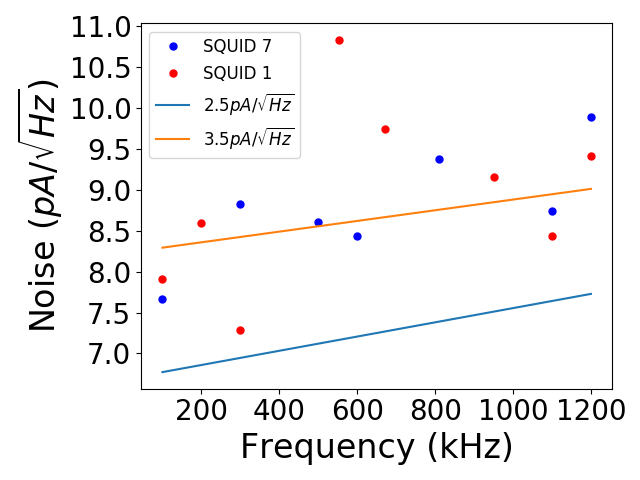
\includegraphics[height=2.5in]{figures/adjusting_squid_noise.png}
\caption{The measured electronic and \ac{SQUID} noise (red and blue dots) as a function of demodulation frequency. The blue line is the noise prediction assuming the intrinsic \ac{SQUID} noise is 2.5~$pA/\sqrt{Hz}$ while the orange line is assuming 3.5~$pA/\sqrt{Hz}$.  
\label{fig:adjust_squid} }
\end{center}
\end{figure}



Demodulating at the bolometer resonant frequencies gave a measure of the 4.2~K bolometers' Johnson noise in addition to the electronic and \ac{SQUID} noise, Figure~\ref{fig:dark_squid_noise}. 
The 4.2~K Johnson noise roughly doubled the noise.
At 770~mK, the low frequency off bolometer resonance noise measured agreed with the prediction but at the higher demodulation frequencies, whether it was on or off resonance, the noise was higher than predicted, Figure~\ref{fig:770mK_squid_noise}. 



\begin{figure}[ht!]
\begin{center}
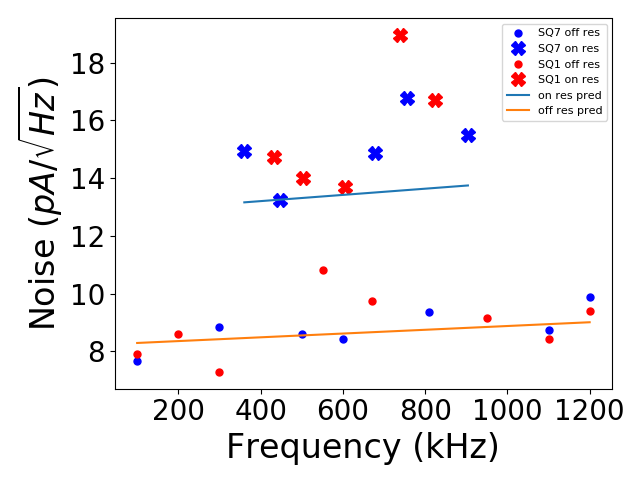
\includegraphics[height=2.5in]{figures/squid_plus_electronic_noise.png}
\caption{Electronic and \ac{SQUID} noise in \ac{ETC} as a function of demodulation frequency at 4.2~K. Off resonance (dots) is just electronic and \ac{SQUID} noise, while on resonance (x's) includes the 4.2~K bolometer Johnson noise. 
\label{fig:dark_squid_noise} }
\end{center}
\end{figure}

\begin{figure}[ht!]
\begin{center}
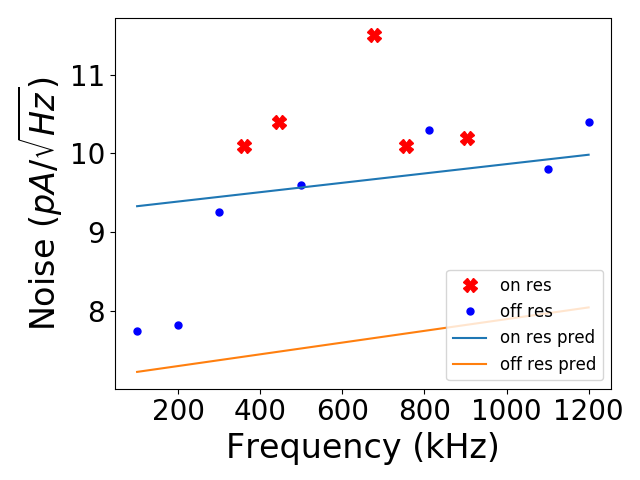
\includegraphics[height=2.5in]{figures/squid_noise_770mK.png}
\caption{Electronic and \ac{SQUID} noise in \ac{ETC} as a function of demodulation frequency at 770~mK. Off resonance (dots) is just electronic and \ac{SQUID} noise, while on resonance (x's) includes the 770~mK bolometer Johnson noise. 
\label{fig:770mK_squid_noise} }
\end{center}
\end{figure}

The measured noise overbiased agreed with the prediction. 
The contribution from the electronics is higher because there are carrier and nullers provided to the bolometer in this measurement. 



\begin{figure}[ht!]
\begin{center}
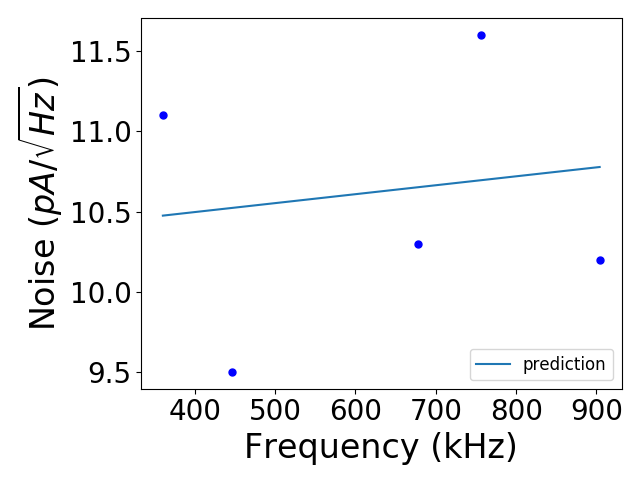
\includegraphics[height=2.5in]{figures/overbias_noise.png}
\caption{Overbias noise (blue dots) for one \ac{SQUID} in \ac{ETC} as a function of demodulation frequency at 340~mK. The prediction (blue line) includes electronic, \ac{SQUID}, and \textcolor{red}{XXX}~mK bolometer Johnson noise. 
\label{fig:overbias_noise} }
\end{center}
\end{figure}



In order to ensure the system was as clean as possible, only \ac{SQUID}7 was tuned. 
There were five bolometers on this comb and we left four overbiased for the in-transition noise measurements. 
Between each measurement, we re-over-biased the bolometer. 
The prediction assumes the bolometer is deep in the transition. 
Deep in the transition, the loopgain, $\mathscr{L}$, is high and so responsivity $S_{I} = \frac{\sqrt{2}}{V_{bias}} \frac{\mathscr{L}}{\mathscr{L}+1} \approx \frac{\sqrt{2}}{V_{bias}} $. 
When the bolometer was not deep in the transition, then $\mathscr{L}$ was not large and so in this case, at high fractions of $R_{initial}$, the phonon noise contribution is over-estimated. 
If $\mathscr{L} = 1$, as is the case at the turnaround of the IV curve near $R = 0.98 \times R_{initial}$, by making this assumption, we overrestimate the phonon contribution by XXX, which decreases the total noise prediction by XXX. 
Even at $R = 0.9 \times R_{initial}$, the high loopgain assumption is not enough to explain the factor of two inconsistency between the measurement and the prediction. 
 

\begin{figure}[ht!]
\begin{center}
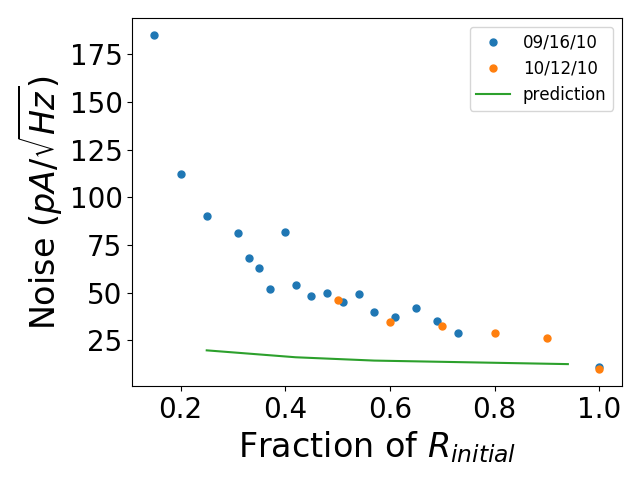
\includegraphics[width=0.48\columnwidth]{figures/b54w2c0_it_noise.png}
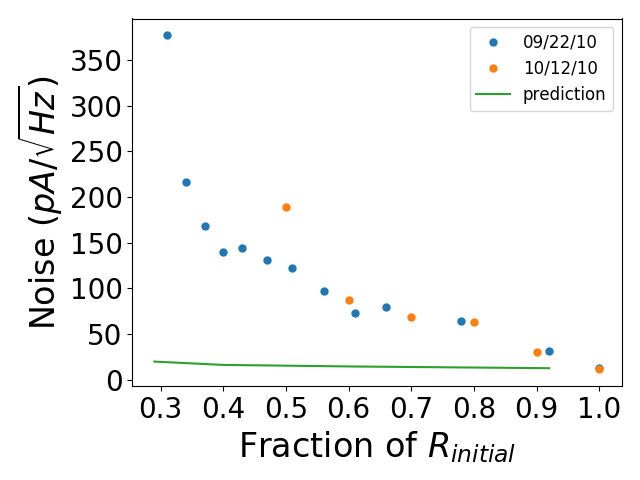
\includegraphics[width=0.48\columnwidth]{figures/b54w2c3_it_noise.png}
\caption{In-transition noise in \ac{ETC} for 150-01 bolometer 3-01 (left) and bolometer 5-02 (right). The prediction (green line) includes electronic, \ac{SQUID}, Johnson, and phonon noise. The measurements were repeatable across multiple days (blue vs orange dots). The overbias noise, at $R_{initial}$, agreed with predictions, but as the depth in transition increased, the discrepancy between the prediction and measurement increased. 
\label{fig:etc_it_noise} }
\end{center}
\end{figure}

The data (blue dot) and prediction (green dot) at $1.0 \times R_{initial}$, i.e. overbiased, agree. 
Note, overbiased, we assume there is no phonon noise contribution. 
Between 0.9 and 0.6 $R_{initial}$, the prediction (green line) assumes the loopgain is large and so there is not modification to the current responsivity, $S_{I}$, for converting the phonon noise from power at the bolometer to current through the \ac{SQUID}.
This assumption is more true at 0.6 and less true at 0.9. 
The measurement at $0.9 \times R_{initial}$ is less than 5\% above the prediction, which includes \ac{SQUID}, electronic, Johnson, and phonon noise. 
At $0.8 \times R_{initial}$, however, the measurement exceeds the prediction by 40\%. 


\begin{figure}[ht!]
\begin{center}
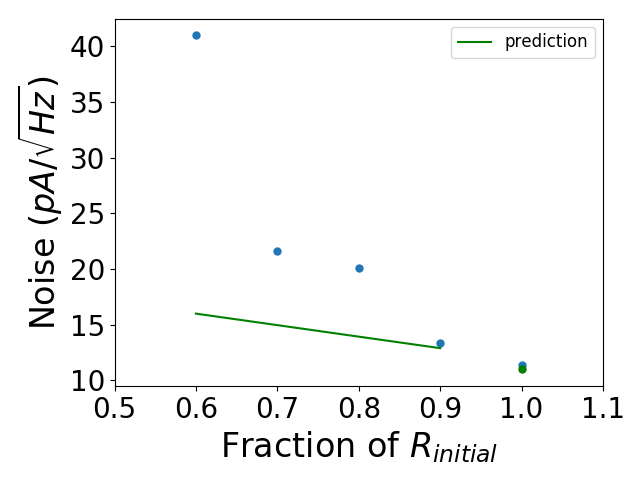
\includegraphics[height=2.5in]{figures/150-02_b53w0c0_it_noise.png}
\caption{150-02 in transition noise for bolometer XXX. 
\label{fig:150-02_it_noise} }
\end{center}
\end{figure}





%%%%%%%%%%%%%%%%%%%%%%%%%%%%%%%%%%%%%%%%%%%%%%%%%%%%%%%%%%%%%%%%%%%%%%%%%%%%%}}}
